\documentclass[]{article}
\usepackage{lmodern}
\usepackage{amssymb,amsmath}
\usepackage{ifxetex,ifluatex}
\usepackage{fixltx2e} % provides \textsubscript
\ifnum 0\ifxetex 1\fi\ifluatex 1\fi=0 % if pdftex
  \usepackage[T1]{fontenc}
  \usepackage[utf8]{inputenc}
\else % if luatex or xelatex
  \ifxetex
    \usepackage{mathspec}
  \else
    \usepackage{fontspec}
  \fi
  \defaultfontfeatures{Ligatures=TeX,Scale=MatchLowercase}
\fi
% use upquote if available, for straight quotes in verbatim environments
\IfFileExists{upquote.sty}{\usepackage{upquote}}{}
% use microtype if available
\IfFileExists{microtype.sty}{%
\usepackage{microtype}
\UseMicrotypeSet[protrusion]{basicmath} % disable protrusion for tt fonts
}{}
\usepackage[margin=1in]{geometry}
\usepackage{hyperref}
\hypersetup{unicode=true,
            pdftitle={Laborator Suplimentar},
            pdfborder={0 0 0},
            breaklinks=true}
\urlstyle{same}  % don't use monospace font for urls
\usepackage{color}
\usepackage{fancyvrb}
\newcommand{\VerbBar}{|}
\newcommand{\VERB}{\Verb[commandchars=\\\{\}]}
\DefineVerbatimEnvironment{Highlighting}{Verbatim}{commandchars=\\\{\}}
% Add ',fontsize=\small' for more characters per line
\usepackage{framed}
\definecolor{shadecolor}{RGB}{248,248,248}
\newenvironment{Shaded}{\begin{snugshade}}{\end{snugshade}}
\newcommand{\KeywordTok}[1]{\textcolor[rgb]{0.13,0.29,0.53}{\textbf{#1}}}
\newcommand{\DataTypeTok}[1]{\textcolor[rgb]{0.13,0.29,0.53}{#1}}
\newcommand{\DecValTok}[1]{\textcolor[rgb]{0.00,0.00,0.81}{#1}}
\newcommand{\BaseNTok}[1]{\textcolor[rgb]{0.00,0.00,0.81}{#1}}
\newcommand{\FloatTok}[1]{\textcolor[rgb]{0.00,0.00,0.81}{#1}}
\newcommand{\ConstantTok}[1]{\textcolor[rgb]{0.00,0.00,0.00}{#1}}
\newcommand{\CharTok}[1]{\textcolor[rgb]{0.31,0.60,0.02}{#1}}
\newcommand{\SpecialCharTok}[1]{\textcolor[rgb]{0.00,0.00,0.00}{#1}}
\newcommand{\StringTok}[1]{\textcolor[rgb]{0.31,0.60,0.02}{#1}}
\newcommand{\VerbatimStringTok}[1]{\textcolor[rgb]{0.31,0.60,0.02}{#1}}
\newcommand{\SpecialStringTok}[1]{\textcolor[rgb]{0.31,0.60,0.02}{#1}}
\newcommand{\ImportTok}[1]{#1}
\newcommand{\CommentTok}[1]{\textcolor[rgb]{0.56,0.35,0.01}{\textit{#1}}}
\newcommand{\DocumentationTok}[1]{\textcolor[rgb]{0.56,0.35,0.01}{\textbf{\textit{#1}}}}
\newcommand{\AnnotationTok}[1]{\textcolor[rgb]{0.56,0.35,0.01}{\textbf{\textit{#1}}}}
\newcommand{\CommentVarTok}[1]{\textcolor[rgb]{0.56,0.35,0.01}{\textbf{\textit{#1}}}}
\newcommand{\OtherTok}[1]{\textcolor[rgb]{0.56,0.35,0.01}{#1}}
\newcommand{\FunctionTok}[1]{\textcolor[rgb]{0.00,0.00,0.00}{#1}}
\newcommand{\VariableTok}[1]{\textcolor[rgb]{0.00,0.00,0.00}{#1}}
\newcommand{\ControlFlowTok}[1]{\textcolor[rgb]{0.13,0.29,0.53}{\textbf{#1}}}
\newcommand{\OperatorTok}[1]{\textcolor[rgb]{0.81,0.36,0.00}{\textbf{#1}}}
\newcommand{\BuiltInTok}[1]{#1}
\newcommand{\ExtensionTok}[1]{#1}
\newcommand{\PreprocessorTok}[1]{\textcolor[rgb]{0.56,0.35,0.01}{\textit{#1}}}
\newcommand{\AttributeTok}[1]{\textcolor[rgb]{0.77,0.63,0.00}{#1}}
\newcommand{\RegionMarkerTok}[1]{#1}
\newcommand{\InformationTok}[1]{\textcolor[rgb]{0.56,0.35,0.01}{\textbf{\textit{#1}}}}
\newcommand{\WarningTok}[1]{\textcolor[rgb]{0.56,0.35,0.01}{\textbf{\textit{#1}}}}
\newcommand{\AlertTok}[1]{\textcolor[rgb]{0.94,0.16,0.16}{#1}}
\newcommand{\ErrorTok}[1]{\textcolor[rgb]{0.64,0.00,0.00}{\textbf{#1}}}
\newcommand{\NormalTok}[1]{#1}
\usepackage{longtable,booktabs}
\usepackage{graphicx,grffile}
\makeatletter
\def\maxwidth{\ifdim\Gin@nat@width>\linewidth\linewidth\else\Gin@nat@width\fi}
\def\maxheight{\ifdim\Gin@nat@height>\textheight\textheight\else\Gin@nat@height\fi}
\makeatother
% Scale images if necessary, so that they will not overflow the page
% margins by default, and it is still possible to overwrite the defaults
% using explicit options in \includegraphics[width, height, ...]{}
\setkeys{Gin}{width=\maxwidth,height=\maxheight,keepaspectratio}
\IfFileExists{parskip.sty}{%
\usepackage{parskip}
}{% else
\setlength{\parindent}{0pt}
\setlength{\parskip}{6pt plus 2pt minus 1pt}
}
\setlength{\emergencystretch}{3em}  % prevent overfull lines
\providecommand{\tightlist}{%
  \setlength{\itemsep}{0pt}\setlength{\parskip}{0pt}}
\setcounter{secnumdepth}{5}
% Redefines (sub)paragraphs to behave more like sections
\ifx\paragraph\undefined\else
\let\oldparagraph\paragraph
\renewcommand{\paragraph}[1]{\oldparagraph{#1}\mbox{}}
\fi
\ifx\subparagraph\undefined\else
\let\oldsubparagraph\subparagraph
\renewcommand{\subparagraph}[1]{\oldsubparagraph{#1}\mbox{}}
\fi

%%% Use protect on footnotes to avoid problems with footnotes in titles
\let\rmarkdownfootnote\footnote%
\def\footnote{\protect\rmarkdownfootnote}

%%% Change title format to be more compact
\usepackage{titling}

% Create subtitle command for use in maketitle
\newcommand{\subtitle}[1]{
  \posttitle{
    \begin{center}\large#1\end{center}
    }
}

\setlength{\droptitle}{-2em}
  \title{Laborator Suplimentar}
  \pretitle{\vspace{\droptitle}\centering\huge}
  \posttitle{\par}
\subtitle{Prezicerea locației într-un sistem de poziționare interior}
  \author{}
  \preauthor{}\postauthor{}
  \date{}
  \predate{}\postdate{}

\usepackage{booktabs}
\usepackage{longtable}
\usepackage{framed,color}
\definecolor{shadecolor}{RGB}{248, 248, 248}
\definecolor{shadecolor1}{RGB}{216,225,235}
\definecolor{framecolor}{RGB}{108,123,13}

\ifxetex
  \usepackage{letltxmacro}
  \setlength{\XeTeXLinkMargin}{1pt}
  \LetLtxMacro\SavedIncludeGraphics\includegraphics
  \def\includegraphics#1#{% #1 catches optional stuff (star/opt. arg.)
    \IncludeGraphicsAux{#1}%
  }%
  \newcommand*{\IncludeGraphicsAux}[2]{%
    \XeTeXLinkBox{%
      \SavedIncludeGraphics#1{#2}%
    }%
  }%
\fi

\newenvironment{frshaded*}{%
  \def\FrameCommand{\fboxrule=\FrameRule\fboxsep=\FrameSep \fcolorbox{framecolor}{shadecolor1}}%
  \MakeFramed {\advance\hsize-\width \FrameRestore}}%
{\endMakeFramed}

\newenvironment{rmdblock}[1]
  {\begin{frshaded*}
  \begin{itemize}
  \renewcommand{\labelitemi}{
    \raisebox{-.7\height}[0pt][0pt]{
      {\setkeys{Gin}{width=2em,keepaspectratio}\includegraphics{images/icons/#1}}
    }
  }
  \item
  }
  {
  \end{itemize}
  \end{frshaded*}
  }
  
\newenvironment{rmdcaution}
  {\begin{rmdblock}{caution}}
  {\end{rmdblock}}
% \newenvironment{rmdinsight}
%   {\begin{rmdblock}{insight}}
%   {\end{rmdblock}}
\newenvironment{rmdexercise}
  {\begin{rmdblock}{exercise}}
  {\end{rmdblock}}
\newenvironment{rmdtip}
  {\begin{rmdblock}{tip}}
  {\end{rmdblock}}
  
  
%%%%%%%%%%%%%%%%%%%%%%%%%%%%%%%%%%%%%%%%%%%%%%%%%%%%%%%%%%%%%%%%%%%%%%%%%%%%%%%%%%%%%%%%%%%%%%%%%%%%%%%%%%%%%%%%%%%%%
%%%%%%%%%%% For insight block %%%%%%%%%%%%%%%%%%%%%%%%%%
\definecolor{shadecolor_insight}{RGB}{223,240,216}
\definecolor{framecolor_insight}{RGB}{136,193,137}

\newenvironment{frshaded_insight*}{%
  \def\FrameCommand{\fboxrule=\FrameRule\fboxsep=\FrameSep \fcolorbox{framecolor_insight}{shadecolor_insight}}%
  \MakeFramed {\advance\hsize-\width \FrameRestore}}%
{\endMakeFramed}

\newenvironment{rmdblock_insight}[1]
  {\begin{frshaded_insight*}
  \begin{itemize}
  \renewcommand{\labelitemi}{
    \raisebox{-.7\height}[0pt][0pt]{
      {\setkeys{Gin}{width=2em,keepaspectratio}\includegraphics{images/icons/#1}}
    }
  }
  \item
  }
  {
  \end{itemize}
  \end{frshaded_insight*}
  }
  
\newenvironment{rmdinsight}
  {\begin{rmdblock_insight}{insight}}
  {\end{rmdblock_insight}}
  
%%%%%%%%%%%%%%%%%%%%%%%%%%%%%%%%%%%%%%%%%%%%%%%%%%%%%%%%%%%%%%%%%%%%%%%%%%%%%%%%%%%%%%%%%%%%%%%%%%%%%%%%%%%%%%%%%%%%%
\usepackage{subfigure}
\usepackage{booktabs}
\usepackage{slashbox}
\usepackage{color}
%%%%%%%%%%%%%%%%%%%%%%%%%%%%%%%%%%%%%%%%%%%%%%%%%%%%%%%%%%%%%%%%%%%%%%%%%%%%%%%%%%%%%%%%%%%%%%%%%%%%%%%%%%%%%%%%%%%%%
%CITEVA DEFINITII
\def\om{\omega}
\def\Om{\Omega}
\def\et{\eta}
\def\td{\tilde{\delta}}
\def\m{{\mu}}
\def\n{{\nu}}
\def\k{{\kappa}}
\def\l{{\lambda}}
\def\L{{\Lambda}}
\def\g{{\gamma}}
\def\a{{\alpha}}
\def\e{{\varepsilon}}
\def\b{{\beta}}
\def\G{{\Gamma}}
\def\d{{\delta}}
\def\D{{\Delta}}
\def\t{{\theta}}
\def\s{{\sigma}}
\def\S{{\Sigma}}
\def\z{{\zeta}}
\def\qed{\hfill\Box}
\def\ds{\displaystyle}
\def\mc{\mathcal}
%%%%%%%%%%%%%%%%%%%%%%%%%%%%%%%%%%%%%%%%%%%%%%%%%%%%%%%%%%%%%%%%%%%%%%%%%%%%%%%%%%%%%%%%%%%%%%%%%%%%%%%%%%%%%%%%%%%%%%
\def\1{{\mathbf 1}}
\def\CC{{\mathbb C}}
\def\VV{{\mathbb V}}
\def\RR{{\mathbb R}}
\def\QQ{{\mathbb Q}}
\def\ZZ{{\mathbb Z}}
\def\PP{{\mathbb P}}
\def\EE{{\mathbb E}}
\def\NN{{\mathbb N}}
\def\FF{{\mathbb F}}
%\def\SS{{\mathbb S}}
\def\MA{{\mathcal A}}
\def\MO{{\mathcal O}}
\def\MF{{\mathcal F}}
\def\ME{{\mathcal E}}
\def\MR{{\mathcal R}}
\def\MB{{\mathcal B}}
\def\MM{{\mathcal M}}
\def\MN{{\mathcal N}}
\def\MU{{\mathcal U}}
\def\MP{{\mathcal P}}
\def\MS{{\mathcal S}}
\def\MBS{{\mathbf S}}
\def\MX{{\bm{ \mathscr X}}}

% independent sign
\newcommand\independent{\protect\mathpalette{\protect\independenT}{\perp}}
\def\independenT#1#2{\mathrel{\rlap{$#1#2$}\mkern2mu{#1#2}}}

\renewcommand{\figurename}{Fig.}

%%%%%%%%%%%%%%%%%%%%%%%%%%%%%%%%%%%%%%%%%%%%%%%%%%%%%%%%%%%%%%%%%%%%%%%%%%%%%%%%%%%%%%%%%%%%%%%%%%%%%%%%%%%%%%%%%%%%%
%Header and Footer
\usepackage{fancyhdr}

\pagestyle{fancy}
\fancyhf{}
\rhead{Universitatea din Bucure\c sti\\ Facultatea de Matematic\u a \c si Informatic\u a}
\lhead{\textit{Curs}: Statistic\u a\\ \textit{Instructori}: A. Am\u arioarei, S. Cojocea}
\rfoot{Pagina \thepage}
\lfoot{Grupele: 301, 311, 321}
%%%%%%%%%%%%%%%%%%%%%%%%%%%%%%%%%%%%%%%
\usepackage{booktabs}
\usepackage{longtable}
\usepackage{array}
\usepackage{multirow}
\usepackage[table]{xcolor}
\usepackage{wrapfig}
\usepackage{float}
\usepackage{colortbl}
\usepackage{pdflscape}
\usepackage{tabu}
\usepackage{threeparttable}

\begin{document}
\maketitle

%%%%%%%%%%%%%%%%%%%%%%%%
\thispagestyle{fancy}

Obiectivul acestui laborator suplimentar este de a prezenta în limbajul
R soluția unei probleme de predicție a locației într-un sistem de
poziționare interior\footnote{Acest laborator este inspirat din lucrarea
  lui Thomas King, Stephan Kopf, Thomas Haenselmann, Christian Lubberger
  și Wolfgang Effelsberg \emph{COMPASS: A probabilistic indoor
  positioning system based on 802.11 and digital compasses}, In
  Proceedings of the 1st international workshop on Wireless network
  testbeds, experimental evaluation characterization (September 2006),
  pp.~34-40 și reproduce parte din capitolul \emph{Predicting location
  via Indoor Positioning Systems} din cartea lui Deborah Nolan și Duncan
  T. Lang \emph{Data Science in R}, CRC Press, 2015}.

\section{Contextul problemei}\label{contextul-problemei}

Scopul acestui exemplu este de a construi un sistem de localizare a
poziției unei persoane în interiorul unei clădiri (IPS - Indoor
Positioning System) pe baza intensității semnalelor WiFi detectate de la
diferite puncte de acces la rețea fixe (access points). Pentru a
construi un astfel de sistem avem nevoie de un set de date de referință
care să conțină informații despre intensitatea semnalului, măsurat în
diferite locații predefinite din interiorul clădirii, dintre un device
mobil (de exemplu un telefon mobil sau un laptop) și diferite puncte de
acces fixe (de exemplu routere). Având aceste date încercăm să construim
un model de localizare a device-ului mobil ca funcție de intensitatea
semnalului dintre acesta și fiecare punct de acces care să permită apoi
prezicerea locației unui nou semnal.

Datele provin din două fișiere .txt, numite
\href{lab_IPS_data/offline.final.trace.txt}{\emph{offline}} și
\href{lab_IPS_data/online.final.trace.txt}{\emph{online}}, care se
găsesc pe site-ul
\href{https://crawdad.org/mannheim/compass/20080411/}{CRAWDAD} (A
Community Resource for Archiving Wireless Data At Dartmouth). Setul de
date \emph{offline} conține măsurători ale intensității semnalului
folosind un laptop IBM Thinkpad R51 pe un grid de 166 de puncte
distanțate la un metru fiecare și distribuite pe o suprafață de
aproximativ 312 \(m^2\) aparținând holului unui birou construit în
campusul Universității din Mannheim (suprafața totală \(15\times 32\) -
vezi planul de mai jos în care cerculețele gri reprezintă locațiile
măsurătorilor offline și pătratele negre sunt locațiile punctelor de
acces - 6).

\begin{center}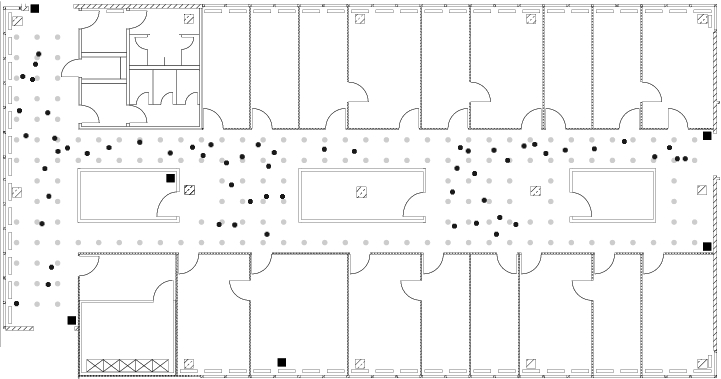
\includegraphics[width=1\linewidth]{lab_IPS_data/building} \end{center}

În plus față de coordonatele \((x,y)\) ale device-ului mobil ne sunt
furnizate și orientările acestuia. Intensitatea semnalelor a fost
înregistrată pentru 8 orientări diferite (0, 45, 90, 135, 180, 225, 270,
315), înregistrându-se un total de 110 măsurători pentru fiecare punct
de acces și fiecare combinație de locație-orientare.

Al doilea set de date, numit \emph{online}, conține 110 înregistrări ale
intensității semnalului măsurate pentru fiecare punct de acces și pentru
60 de locații și orientări alese aleator. Acest set de date va fi
folosit pentru prezicerea poziției unui device mobil.

În ambele seturi de date, \emph{offline} și \emph{online}, o parte din
cele 110 intensități de semnale nu au fost înregistrate și în plus pot
apărea și măsurători de la alte device-uri din vecinătatea unității
experimentale (e.g.~de la alte laptop-uri sau telefoane).

\section{Descrierea și curățarea
datelor}\label{descrierea-si-curatarea-datelor}

În această etapă vom preprocesa datele din formatul raw (neprelucrat) și
le vom explora în vederea analizei ulterioare. Dacă deschidem fișierul
\emph{offline.final.trace.txt} cu ajutorul unui editor de text (de
exemplu \href{https://notepad-plus-plus.org/}{Notepad++}) putem vedea
forma generală a înregistrărilor pentru a ne face o imagine preliminară
asupra acestora. O primă intrare este de forma:

\begin{verbatim}
 [1] "# timestamp=2006-02-11 08:31:58"   
 [2] "# usec=250"                        
 [3] "# minReadings=110"                 
 [4] "t=1139643118358"                   
 [5] "id=00:02:2D:21:0F:33"              
 [6] "pos=0.0,0.0,0.0"                   
 [7] "degree=0.0"                        
 [8] "00:14:bf:b1:97:8a=-38,2437000000,3"
 [9] "00:14:bf:b1:97:90=-56,2427000000,3"
[10] "00:0f:a3:39:e1:c0=-53,2462000000,3"
[11] "00:14:bf:b1:97:8d=-65,2442000000,3"
[12] "00:14:bf:b1:97:81=-65,2422000000,3"
[13] "00:14:bf:3b:c7:c6=-66,2432000000,3"
[14] "00:0f:a3:39:dd:cd=-75,2412000000,3"
[15] "00:0f:a3:39:e0:4b=-78,2462000000,3"
[16] "00:0f:a3:39:e2:10=-87,2437000000,3"
[17] "02:64:fb:68:52:e6=-88,2447000000,1"
[18] "02:00:42:55:31:00=-84,2457000000,1"
\end{verbatim}

Tabelul de mai jos prezintă descrierea variabilelor care apar în
seturile de date \emph{offline} și \emph{online}:

\begin{longtable}[]{@{}ll@{}}
\toprule
\begin{minipage}[b]{0.10\columnwidth}\raggedright\strut
Variabila\strut
\end{minipage} & \begin{minipage}[b]{0.63\columnwidth}\raggedright\strut
Scurtă descriere\strut
\end{minipage}\tabularnewline
\midrule
\endhead
\begin{minipage}[t]{0.10\columnwidth}\raggedright\strut
t\strut
\end{minipage} & \begin{minipage}[t]{0.63\columnwidth}\raggedright\strut
timestamp-ul calculată în milisecunde de la miezul nopții zilei de 1
Ianuarie 1970\strut
\end{minipage}\tabularnewline
\begin{minipage}[t]{0.10\columnwidth}\raggedright\strut
id\strut
\end{minipage} & \begin{minipage}[t]{0.63\columnwidth}\raggedright\strut
adresa MAC a device-ului cu care s-a scanat\strut
\end{minipage}\tabularnewline
\begin{minipage}[t]{0.10\columnwidth}\raggedright\strut
pos\strut
\end{minipage} & \begin{minipage}[t]{0.63\columnwidth}\raggedright\strut
poziția fizică a device-ului cu care s-a scanat\strut
\end{minipage}\tabularnewline
\begin{minipage}[t]{0.10\columnwidth}\raggedright\strut
degree\strut
\end{minipage} & \begin{minipage}[t]{0.63\columnwidth}\raggedright\strut
unghiul de orientare a device-ului cu care s-a scanat\strut
\end{minipage}\tabularnewline
\begin{minipage}[t]{0.10\columnwidth}\raggedright\strut
MAC\strut
\end{minipage} & \begin{minipage}[t]{0.63\columnwidth}\raggedright\strut
adresa MAC a unui device respondent cu valoarea intensității semnalului
în dBm, frecvența canalului și tipul acestuia (punct de acces = 3 și
device adhoc = 1)\strut
\end{minipage}\tabularnewline
\bottomrule
\end{longtable}

Deoarece datele nu vin într-un format bine definit le vom citi fișierul
\emph{offline.final.trace.txt} cu ajutorul funcției \texttt{readLines()}
și apoi ne vom uita la numărul de linii care încep cu \(\#\):

\begin{Shaded}
\begin{Highlighting}[]
\NormalTok{doc =}\StringTok{ }\KeywordTok{readLines}\NormalTok{(}\StringTok{"lab_IPS_data/offline.final.trace.txt"}\NormalTok{)}
\KeywordTok{sum}\NormalTok{(}\KeywordTok{substr}\NormalTok{(doc,}\DecValTok{1}\NormalTok{,}\DecValTok{1}\NormalTok{) }\OperatorTok{==}\StringTok{ "#"}\NormalTok{) }\CommentTok{# nr de linii care incep cu "#"}
\NormalTok{[}\DecValTok{1}\NormalTok{] }\DecValTok{5312}
\KeywordTok{length}\NormalTok{(doc) }\CommentTok{# cate linii are documentul}
\NormalTok{[}\DecValTok{1}\NormalTok{] }\DecValTok{151392}

\CommentTok{# cate linii avem de fapt }
\CommentTok{# coincide cu nr pe care ne asteptam sa-l avem }
\KeywordTok{length}\NormalTok{(doc) }\OperatorTok{-}\StringTok{ }\KeywordTok{sum}\NormalTok{(}\KeywordTok{substr}\NormalTok{(doc,}\DecValTok{1}\NormalTok{,}\DecValTok{1}\NormalTok{) }\OperatorTok{==}\StringTok{ "#"}\NormalTok{) }
\NormalTok{[}\DecValTok{1}\NormalTok{] }\DecValTok{146080}
\CommentTok{# ne asteptam la }
\DecValTok{166}\OperatorTok{*}\DecValTok{8}\OperatorTok{*}\DecValTok{110} 
\NormalTok{[}\DecValTok{1}\NormalTok{] }\DecValTok{146080}
\end{Highlighting}
\end{Shaded}

\subsection{Preprocesarea datelor}\label{preprocesarea-datelor}

În această secțiune vrem să scriem o funcție care să permită
transformarea datelor din formatul brut într-un format tabelar (un
data.frame) care să aibă drept coloane variabile precum timpul (time),
id-ul adresei MAC a device-ului cu care am scanat (mac-id), locația
device-ului (coordonatele \(x,y,z\)), orientarea device-ului, adresa MAC
a emitentului semnalului, intensitatea semnalului, frecvența canalului
de transmitere precum și tipul de emitent (punct de acces sau device
adhoc).

Dacă ne uităm la prima intrare din setul de date \emph{offline} care nu
este un comentariu (nu începe cu \(\#\)) atunci observăm că numele
variabilei este separat de valoarea acesteia prin semnul \(=\) iar în
situații precum poziția valorile sunt separate prin \(,\):

\begin{Shaded}
\begin{Highlighting}[]
\KeywordTok{strsplit}\NormalTok{(doc[}\DecValTok{4}\NormalTok{], }\StringTok{";"}\NormalTok{)[[}\DecValTok{1}\NormalTok{]]}
\NormalTok{ [}\DecValTok{1}\NormalTok{] }\StringTok{"t=1139643118358"}                   
\NormalTok{ [}\DecValTok{2}\NormalTok{] }\StringTok{"id=00:02:2D:21:0F:33"}              
\NormalTok{ [}\DecValTok{3}\NormalTok{] }\StringTok{"pos=0.0,0.0,0.0"}                   
\NormalTok{ [}\DecValTok{4}\NormalTok{] }\StringTok{"degree=0.0"}                        
\NormalTok{ [}\DecValTok{5}\NormalTok{] }\StringTok{"00:14:bf:b1:97:8a=-38,2437000000,3"}
\NormalTok{ [}\DecValTok{6}\NormalTok{] }\StringTok{"00:14:bf:b1:97:90=-56,2427000000,3"}
\NormalTok{ [}\DecValTok{7}\NormalTok{] }\StringTok{"00:0f:a3:39:e1:c0=-53,2462000000,3"}
\NormalTok{ [}\DecValTok{8}\NormalTok{] }\StringTok{"00:14:bf:b1:97:8d=-65,2442000000,3"}
\NormalTok{ [}\DecValTok{9}\NormalTok{] }\StringTok{"00:14:bf:b1:97:81=-65,2422000000,3"}
\NormalTok{[}\DecValTok{10}\NormalTok{] }\StringTok{"00:14:bf:3b:c7:c6=-66,2432000000,3"}
\NormalTok{[}\DecValTok{11}\NormalTok{] }\StringTok{"00:0f:a3:39:dd:cd=-75,2412000000,3"}
\NormalTok{[}\DecValTok{12}\NormalTok{] }\StringTok{"00:0f:a3:39:e0:4b=-78,2462000000,3"}
\NormalTok{[}\DecValTok{13}\NormalTok{] }\StringTok{"00:0f:a3:39:e2:10=-87,2437000000,3"}
\NormalTok{[}\DecValTok{14}\NormalTok{] }\StringTok{"02:64:fb:68:52:e6=-88,2447000000,1"}
\NormalTok{[}\DecValTok{15}\NormalTok{] }\StringTok{"02:00:42:55:31:00=-84,2457000000,1"}
\end{Highlighting}
\end{Shaded}

Pentru a separa șirul de caractere \texttt{doc{[}4{]}} în funcție de
\(;\), \(=\) sau \(,\) folosim expresia regulată \texttt{{[};=,{]}} ca
argument a funcției \texttt{strsplit()}:

\begin{Shaded}
\begin{Highlighting}[]
\NormalTok{tokens =}\StringTok{ }\KeywordTok{strsplit}\NormalTok{(doc[}\DecValTok{4}\NormalTok{], }\StringTok{"[;=,]"}\NormalTok{)[[}\DecValTok{1}\NormalTok{]]}
\NormalTok{tokens[}\KeywordTok{c}\NormalTok{(}\DecValTok{2}\NormalTok{,}\DecValTok{4}\NormalTok{,}\DecValTok{6}\OperatorTok{:}\DecValTok{8}\NormalTok{, }\DecValTok{10}\NormalTok{)] }\CommentTok{# doar valorile primelor 6 variabile}
\NormalTok{[}\DecValTok{1}\NormalTok{] }\StringTok{"1139643118358"}     \StringTok{"00:02:2D:21:0F:33"} \StringTok{"0.0"}              
\NormalTok{[}\DecValTok{4}\NormalTok{] }\StringTok{"0.0"}               \StringTok{"0.0"}               \StringTok{"0.0"}              

\CommentTok{# pt celelalte 4 variabile: MAC, signal, channel, device type}
\NormalTok{tokens[}\OperatorTok{-}\NormalTok{(}\DecValTok{1}\OperatorTok{:}\DecValTok{10}\NormalTok{)]}
\NormalTok{ [}\DecValTok{1}\NormalTok{] }\StringTok{"00:14:bf:b1:97:8a"} \StringTok{"-38"}               \StringTok{"2437000000"}       
\NormalTok{ [}\DecValTok{4}\NormalTok{] }\StringTok{"3"}                 \StringTok{"00:14:bf:b1:97:90"} \StringTok{"-56"}              
\NormalTok{ [}\DecValTok{7}\NormalTok{] }\StringTok{"2427000000"}        \StringTok{"3"}                 \StringTok{"00:0f:a3:39:e1:c0"}
\NormalTok{[}\DecValTok{10}\NormalTok{] }\StringTok{"-53"}               \StringTok{"2462000000"}        \StringTok{"3"}                
\NormalTok{[}\DecValTok{13}\NormalTok{] }\StringTok{"00:14:bf:b1:97:8d"} \StringTok{"-65"}               \StringTok{"2442000000"}       
\NormalTok{[}\DecValTok{16}\NormalTok{] }\StringTok{"3"}                 \StringTok{"00:14:bf:b1:97:81"} \StringTok{"-65"}              
\NormalTok{[}\DecValTok{19}\NormalTok{] }\StringTok{"2422000000"}        \StringTok{"3"}                 \StringTok{"00:14:bf:3b:c7:c6"}
\NormalTok{[}\DecValTok{22}\NormalTok{] }\StringTok{"-66"}               \StringTok{"2432000000"}        \StringTok{"3"}                
\NormalTok{[}\DecValTok{25}\NormalTok{] }\StringTok{"00:0f:a3:39:dd:cd"} \StringTok{"-75"}               \StringTok{"2412000000"}       
\NormalTok{[}\DecValTok{28}\NormalTok{] }\StringTok{"3"}                 \StringTok{"00:0f:a3:39:e0:4b"} \StringTok{"-78"}              
\NormalTok{[}\DecValTok{31}\NormalTok{] }\StringTok{"2462000000"}        \StringTok{"3"}                 \StringTok{"00:0f:a3:39:e2:10"}
\NormalTok{[}\DecValTok{34}\NormalTok{] }\StringTok{"-87"}               \StringTok{"2437000000"}        \StringTok{"3"}                
\NormalTok{[}\DecValTok{37}\NormalTok{] }\StringTok{"02:64:fb:68:52:e6"} \StringTok{"-88"}               \StringTok{"2447000000"}       
\NormalTok{[}\DecValTok{40}\NormalTok{] }\StringTok{"1"}                 \StringTok{"02:00:42:55:31:00"} \StringTok{"-84"}              
\NormalTok{[}\DecValTok{43}\NormalTok{] }\StringTok{"2457000000"}        \StringTok{"1"}                
\end{Highlighting}
\end{Shaded}

Valorile din \texttt{tokens{[}-(1:10){]}} pot fi văzute ca o matrice cu
4 coloane și câte un rând pentru fiecare adresă de MAC emitentă.
Următoarea funcție înglobează aceste operații în vederea aplicârii ei pe
întreg setul de date (mai exact pentru fiecare rând din setul de date
\emph{offline}). Ea conține de asemenea și cazul în care sunt intrări în
setul de date care nu au niciun semnal:

\begin{Shaded}
\begin{Highlighting}[]
\NormalTok{processLine =}\StringTok{ }\ControlFlowTok{function}\NormalTok{(x)\{}
  \CommentTok{# x este linia documentului }
  \CommentTok{# luam in considerare liniile mai scurte - cele care au mai }
  \CommentTok{# putin de 10 variabile (nu avem observatii de semnal)}
\NormalTok{  tokens =}\StringTok{ }\KeywordTok{strsplit}\NormalTok{(x, }\StringTok{"[;=,]"}\NormalTok{)[[}\DecValTok{1}\NormalTok{]]}
  \CommentTok{# pt obs care au 10 obs}
  \ControlFlowTok{if}\NormalTok{ (}\KeywordTok{length}\NormalTok{(tokens) }\OperatorTok{==}\StringTok{ }\DecValTok{10}\NormalTok{)\{}
    \KeywordTok{return}\NormalTok{(}\OtherTok{NULL}\NormalTok{)}
\NormalTok{  \}}
  
\NormalTok{  tmp =}\StringTok{ }\KeywordTok{matrix}\NormalTok{(tokens[}\OperatorTok{-}\NormalTok{(}\DecValTok{1}\OperatorTok{:}\DecValTok{10}\NormalTok{)], }\DataTypeTok{ncol =} \DecValTok{4}\NormalTok{, }\DataTypeTok{byrow =} \OtherTok{TRUE}\NormalTok{)}
  \KeywordTok{cbind}\NormalTok{(}\KeywordTok{matrix}\NormalTok{(tokens[}\KeywordTok{c}\NormalTok{(}\DecValTok{2}\NormalTok{,}\DecValTok{4}\NormalTok{,}\DecValTok{6}\OperatorTok{:}\DecValTok{8}\NormalTok{, }\DecValTok{10}\NormalTok{)], }
               \DataTypeTok{nrow =} \KeywordTok{nrow}\NormalTok{(tmp), }\DataTypeTok{ncol =} \DecValTok{6}\NormalTok{, }\DataTypeTok{byrow =} \OtherTok{TRUE}\NormalTok{),tmp)}
\NormalTok{\}}
\end{Highlighting}
\end{Shaded}

Apelăm această funcție pe întreg setul de date:

\begin{Shaded}
\begin{Highlighting}[]
\CommentTok{# stergem liniile cu # din setul de date}
\NormalTok{lines =}\StringTok{ }\NormalTok{doc[}\KeywordTok{substr}\NormalTok{(doc, }\DecValTok{1}\NormalTok{, }\DecValTok{1}\NormalTok{) }\OperatorTok{!=}\StringTok{ "#"}\NormalTok{]}

\NormalTok{tmp =}\StringTok{ }\KeywordTok{lapply}\NormalTok{(lines, processLine) }\CommentTok{# procesam fiecare linie din doc}

\CommentTok{# combina data intr-un data.frame }
\CommentTok{# uneste toate matricele din lista obtinuta folosind do.call()}
\NormalTok{offline =}\StringTok{ }\KeywordTok{as.data.frame}\NormalTok{(}\KeywordTok{do.call}\NormalTok{(}\StringTok{"rbind"}\NormalTok{, tmp), }
                        \DataTypeTok{stringsAsFactors =} \OtherTok{FALSE}\NormalTok{)}

\KeywordTok{str}\NormalTok{(offline)}
\StringTok{'data.frame'}\OperatorTok{:}\StringTok{   }\DecValTok{1181628}\NormalTok{ obs. of  }\DecValTok{10}\NormalTok{ variables}\OperatorTok{:}
\StringTok{ }\ErrorTok{$}\StringTok{ }\NormalTok{V1 }\OperatorTok{:}\StringTok{ }\NormalTok{chr  }\StringTok{"1139643118358"} \StringTok{"1139643118358"} \StringTok{"1139643118358"} \StringTok{"1139643118358"}\NormalTok{ ...}
 \OperatorTok{$}\StringTok{ }\NormalTok{V2 }\OperatorTok{:}\StringTok{ }\NormalTok{chr  }\StringTok{"00:02:2D:21:0F:33"} \StringTok{"00:02:2D:21:0F:33"} \StringTok{"00:02:2D:21:0F:33"} \StringTok{"00:02:2D:21:0F:33"}\NormalTok{ ...}
 \OperatorTok{$}\StringTok{ }\NormalTok{V3 }\OperatorTok{:}\StringTok{ }\NormalTok{chr  }\StringTok{"0.0"} \StringTok{"0.0"} \StringTok{"0.0"} \StringTok{"0.0"}\NormalTok{ ...}
 \OperatorTok{$}\StringTok{ }\NormalTok{V4 }\OperatorTok{:}\StringTok{ }\NormalTok{chr  }\StringTok{"0.0"} \StringTok{"0.0"} \StringTok{"0.0"} \StringTok{"0.0"}\NormalTok{ ...}
 \OperatorTok{$}\StringTok{ }\NormalTok{V5 }\OperatorTok{:}\StringTok{ }\NormalTok{chr  }\StringTok{"0.0"} \StringTok{"0.0"} \StringTok{"0.0"} \StringTok{"0.0"}\NormalTok{ ...}
 \OperatorTok{$}\StringTok{ }\NormalTok{V6 }\OperatorTok{:}\StringTok{ }\NormalTok{chr  }\StringTok{"0.0"} \StringTok{"0.0"} \StringTok{"0.0"} \StringTok{"0.0"}\NormalTok{ ...}
 \OperatorTok{$}\StringTok{ }\NormalTok{V7 }\OperatorTok{:}\StringTok{ }\NormalTok{chr  }\StringTok{"00:14:bf:b1:97:8a"} \StringTok{"00:14:bf:b1:97:90"} \StringTok{"00:0f:a3:39:e1:c0"} \StringTok{"00:14:bf:b1:97:8d"}\NormalTok{ ...}
 \OperatorTok{$}\StringTok{ }\NormalTok{V8 }\OperatorTok{:}\StringTok{ }\NormalTok{chr  }\StringTok{"-38"} \StringTok{"-56"} \StringTok{"-53"} \StringTok{"-65"}\NormalTok{ ...}
 \OperatorTok{$}\StringTok{ }\NormalTok{V9 }\OperatorTok{:}\StringTok{ }\NormalTok{chr  }\StringTok{"2437000000"} \StringTok{"2427000000"} \StringTok{"2462000000"} \StringTok{"2442000000"}\NormalTok{ ...}
 \OperatorTok{$}\StringTok{ }\NormalTok{V10}\OperatorTok{:}\StringTok{ }\NormalTok{chr  }\StringTok{"3"} \StringTok{"3"} \StringTok{"3"} \StringTok{"3"}\NormalTok{ ...}
\end{Highlighting}
\end{Shaded}

Cum data.frame-ul obținut conține numai variabile de tip
\texttt{character} următorul pas constă în transformarea acestora după
tipul corespunzător, e.g.~intensitatea semnalului să devină
\texttt{numeric}.

\begin{Shaded}
\begin{Highlighting}[]
\CommentTok{# dam nume variabilelor}
\KeywordTok{names}\NormalTok{(offline) =}\StringTok{ }\KeywordTok{c}\NormalTok{(}\StringTok{"time"}\NormalTok{,}\StringTok{"scanMac"}\NormalTok{, }\StringTok{"posX"}\NormalTok{, }\StringTok{"posY"}\NormalTok{, }\StringTok{"posZ"}\NormalTok{, }
                   \StringTok{"orientation"}\NormalTok{, }\StringTok{"mac"}\NormalTok{, }\StringTok{"signal"}\NormalTok{, }\StringTok{"channel"}\NormalTok{, }\StringTok{"type"}\NormalTok{)}

\CommentTok{# convertim variabilele numerice}
\NormalTok{numVars =}\StringTok{ }\KeywordTok{c}\NormalTok{(}\StringTok{"time"}\NormalTok{, }\StringTok{"posX"}\NormalTok{, }\StringTok{"posY"}\NormalTok{, }\StringTok{"posZ"}\NormalTok{, }\StringTok{"orientation"}\NormalTok{,  }\StringTok{"signal"}\NormalTok{)}
\NormalTok{offline[numVars] =}\StringTok{ }\KeywordTok{lapply}\NormalTok{(offline[numVars], as.numeric)}
\end{Highlighting}
\end{Shaded}

Cum suntem interasați doar de semnale care provin de la punctele de
acces putem să eliminăm înregistrările care conțin adrese de la
device-uri adhoc (\texttt{type\ =\ 3}).

\begin{Shaded}
\begin{Highlighting}[]
\NormalTok{offline =}\StringTok{ }\NormalTok{offline[offline}\OperatorTok{$}\NormalTok{type }\OperatorTok{==}\StringTok{ "3"}\NormalTok{, ]}

\CommentTok{# stergem variabila type}
\NormalTok{offline =}\StringTok{ }\NormalTok{offline[ , }\KeywordTok{names}\NormalTok{(offline) }\OperatorTok{!=}\StringTok{ "type"}\NormalTok{] }
\KeywordTok{dim}\NormalTok{(offline)}
\NormalTok{[}\DecValTok{1}\NormalTok{] }\DecValTok{978443}      \DecValTok{9}
\end{Highlighting}
\end{Shaded}

Dacă ne uităm la variabila \texttt{time} și ținem cont de descrierea din
tabelul de mai sus putem să o transformăm în formatul \texttt{POSIXt}
pentru a putea ulterior să efectuăm operații cu ea în R (să remarcăm
totuși că timpul în setul de date este măsurat în milisecunde față de
data de referință 01.01.1970 iar în formatul amintit timpul este măsurat
față de aceeași dată de referință numai că în secunde, deci se impune o
transformare):

\begin{Shaded}
\begin{Highlighting}[]
\NormalTok{offline}\OperatorTok{$}\NormalTok{rawTime =}\StringTok{ }\NormalTok{offline}\OperatorTok{$}\NormalTok{time}
\CommentTok{# transformam timpul din millisecunde in secunde}
\NormalTok{offline}\OperatorTok{$}\NormalTok{time =}\StringTok{ }\NormalTok{offline}\OperatorTok{$}\NormalTok{time}\OperatorTok{/}\DecValTok{1000}  
\KeywordTok{class}\NormalTok{(offline}\OperatorTok{$}\NormalTok{time) =}\StringTok{ }\KeywordTok{c}\NormalTok{(}\StringTok{"POSIXt"}\NormalTok{, }\StringTok{"POSIXct"}\NormalTok{)}
\end{Highlighting}
\end{Shaded}

Vrem să verificăm cum arată fiecare variabilă din setul de date aplicând
funcția \texttt{summary} (pentru variabile de tip caracter trebuie să le
transformăm în prealabil în date de tip \texttt{factor} pentru a putea
aplica funcția \texttt{summary} și în acest caz obținem câte observații
avem din fiecare valoarea unică a variabilelor calitative avem):

\begin{Shaded}
\begin{Highlighting}[]
\CommentTok{# variabilele numerice}
\KeywordTok{summary}\NormalTok{(offline[, numVars])}
\NormalTok{      time                          posX            posY       }
\NormalTok{ Min.   }\OperatorTok{:}\DecValTok{2006}\OperatorTok{-}\DecValTok{02}\OperatorTok{-}\DecValTok{11} \DecValTok{09}\OperatorTok{:}\DecValTok{31}\OperatorTok{:}\DecValTok{58}\NormalTok{   Min.   }\OperatorTok{:}\StringTok{ }\FloatTok{0.00}\NormalTok{   Min.   }\OperatorTok{:}\StringTok{ }\FloatTok{0.000}  
\NormalTok{ 1st Qu.}\OperatorTok{:}\DecValTok{2006}\OperatorTok{-}\DecValTok{02}\OperatorTok{-}\DecValTok{11} \DecValTok{15}\OperatorTok{:}\DecValTok{21}\OperatorTok{:}\DecValTok{27}\NormalTok{   1st Qu.}\OperatorTok{:}\StringTok{ }\FloatTok{2.00}\NormalTok{   1st Qu.}\OperatorTok{:}\StringTok{ }\FloatTok{3.000}  
\NormalTok{ Median }\OperatorTok{:}\DecValTok{2006}\OperatorTok{-}\DecValTok{02}\OperatorTok{-}\DecValTok{11} \DecValTok{21}\OperatorTok{:}\DecValTok{57}\OperatorTok{:}\DecValTok{58}\NormalTok{   Median }\OperatorTok{:}\FloatTok{12.00}\NormalTok{   Median }\OperatorTok{:}\StringTok{ }\FloatTok{6.000}  
\NormalTok{ Mean   }\OperatorTok{:}\DecValTok{2006}\OperatorTok{-}\DecValTok{02}\OperatorTok{-}\DecValTok{16} \DecValTok{16}\OperatorTok{:}\DecValTok{57}\OperatorTok{:}\DecValTok{37}\NormalTok{   Mean   }\OperatorTok{:}\FloatTok{13.52}\NormalTok{   Mean   }\OperatorTok{:}\StringTok{ }\FloatTok{5.897}  
\NormalTok{ 3rd Qu.}\OperatorTok{:}\DecValTok{2006}\OperatorTok{-}\DecValTok{02}\OperatorTok{-}\DecValTok{19} \DecValTok{16}\OperatorTok{:}\DecValTok{52}\OperatorTok{:}\DecValTok{40}\NormalTok{   3rd Qu.}\OperatorTok{:}\FloatTok{23.00}\NormalTok{   3rd Qu.}\OperatorTok{:}\StringTok{ }\FloatTok{8.000}  
\NormalTok{ Max.   }\OperatorTok{:}\DecValTok{2006}\OperatorTok{-}\DecValTok{03}\OperatorTok{-}\DecValTok{09} \DecValTok{22}\OperatorTok{:}\DecValTok{41}\OperatorTok{:}\DecValTok{10}\NormalTok{   Max.   }\OperatorTok{:}\FloatTok{33.00}\NormalTok{   Max.   }\OperatorTok{:}\FloatTok{13.000}  
\NormalTok{      posZ    orientation        signal     }
\NormalTok{ Min.   }\OperatorTok{:}\DecValTok{0}\NormalTok{   Min.   }\OperatorTok{:}\StringTok{  }\FloatTok{0.0}\NormalTok{   Min.   }\OperatorTok{:-}\FloatTok{99.0}  
\NormalTok{ 1st Qu.}\OperatorTok{:}\DecValTok{0}\NormalTok{   1st Qu.}\OperatorTok{:}\StringTok{ }\FloatTok{90.0}\NormalTok{   1st Qu.}\OperatorTok{:-}\FloatTok{69.0}  
\NormalTok{ Median }\OperatorTok{:}\DecValTok{0}\NormalTok{   Median }\OperatorTok{:}\FloatTok{180.0}\NormalTok{   Median }\OperatorTok{:-}\FloatTok{60.0}  
\NormalTok{ Mean   }\OperatorTok{:}\DecValTok{0}\NormalTok{   Mean   }\OperatorTok{:}\FloatTok{167.2}\NormalTok{   Mean   }\OperatorTok{:-}\FloatTok{61.7}  
\NormalTok{ 3rd Qu.}\OperatorTok{:}\DecValTok{0}\NormalTok{   3rd Qu.}\OperatorTok{:}\FloatTok{270.0}\NormalTok{   3rd Qu.}\OperatorTok{:-}\FloatTok{53.0}  
\NormalTok{ Max.   }\OperatorTok{:}\DecValTok{0}\NormalTok{   Max.   }\OperatorTok{:}\FloatTok{359.9}\NormalTok{   Max.   }\OperatorTok{:-}\FloatTok{25.0}  

\CommentTok{# variabilele calitative - trebuie transformate in factor}
\KeywordTok{summary}\NormalTok{(}\KeywordTok{sapply}\NormalTok{(offline[, }\KeywordTok{c}\NormalTok{(}\StringTok{"mac"}\NormalTok{, }\StringTok{"channel"}\NormalTok{, }\StringTok{"scanMac"}\NormalTok{)], }
\NormalTok{               as.factor))}
\NormalTok{                mac               channel                    scanMac      }
 \DecValTok{00}\OperatorTok{:}\NormalTok{0f}\OperatorTok{:}\NormalTok{a3}\OperatorTok{:}\DecValTok{39}\OperatorTok{:}\NormalTok{e1}\OperatorTok{:}\NormalTok{c0}\OperatorTok{:}\DecValTok{145862}   \DecValTok{2462000000}\OperatorTok{:}\DecValTok{189774}   \DecValTok{00}\OperatorTok{:}\DecValTok{02}\OperatorTok{:}\NormalTok{2D}\OperatorTok{:}\DecValTok{21}\OperatorTok{:}\NormalTok{0F}\OperatorTok{:}\DecValTok{33}\OperatorTok{:}\DecValTok{978443}  
 \DecValTok{00}\OperatorTok{:}\NormalTok{0f}\OperatorTok{:}\NormalTok{a3}\OperatorTok{:}\DecValTok{39}\OperatorTok{:}\NormalTok{dd}\OperatorTok{:}\NormalTok{cd}\OperatorTok{:}\DecValTok{145619}   \DecValTok{2437000000}\OperatorTok{:}\DecValTok{152124}                             
 \DecValTok{00}\OperatorTok{:}\DecValTok{14}\OperatorTok{:}\NormalTok{bf}\OperatorTok{:}\NormalTok{b1}\OperatorTok{:}\DecValTok{97}\OperatorTok{:}\NormalTok{8a}\OperatorTok{:}\DecValTok{132962}   \DecValTok{2412000000}\OperatorTok{:}\DecValTok{145619}                             
 \DecValTok{00}\OperatorTok{:}\DecValTok{14}\OperatorTok{:}\NormalTok{bf}\OperatorTok{:}\NormalTok{3b}\OperatorTok{:}\NormalTok{c7}\OperatorTok{:}\NormalTok{c6}\OperatorTok{:}\DecValTok{126529}   \DecValTok{2432000000}\OperatorTok{:}\DecValTok{126529}                             
 \DecValTok{00}\OperatorTok{:}\DecValTok{14}\OperatorTok{:}\NormalTok{bf}\OperatorTok{:}\NormalTok{b1}\OperatorTok{:}\DecValTok{97}\OperatorTok{:}\DecValTok{90}\OperatorTok{:}\DecValTok{122315}   \DecValTok{2427000000}\OperatorTok{:}\DecValTok{122315}                             
 \DecValTok{00}\OperatorTok{:}\DecValTok{14}\OperatorTok{:}\NormalTok{bf}\OperatorTok{:}\NormalTok{b1}\OperatorTok{:}\DecValTok{97}\OperatorTok{:}\NormalTok{8d}\OperatorTok{:}\DecValTok{121325}   \DecValTok{2442000000}\OperatorTok{:}\DecValTok{121325}                             
\NormalTok{ (Other)          }\OperatorTok{:}\DecValTok{183831}\NormalTok{   (Other)   }\OperatorTok{:}\DecValTok{120757}                             
\end{Highlighting}
\end{Shaded}

Uitându-ne la rezultatele obținute mai sus remarcăm că variabila
\texttt{scanMac} are o singură valoarea ceea ce ne spune că datele au
fost culese cu un singur aparat și prin urmare putem să renunțăm la
această variabilă. De asemenea variabila \texttt{posZ} este constantă
\(0\) ceea ce înseamnă că toate măsurătorile au fost luate de la același
nivel și putem renunța și la această variabilă.

\begin{Shaded}
\begin{Highlighting}[]
\NormalTok{offline =}\StringTok{ }\NormalTok{offline[, }\OperatorTok{!}\KeywordTok{names}\NormalTok{(offline) }\OperatorTok\StringTok{ }\KeywordTok{c}\NormalTok{(}\StringTok{"scanMac"}\NormalTok{, }\StringTok{"posZ"}\NormalTok{)]}
\end{Highlighting}
\end{Shaded}

\subsection{Să explorăm orientările}\label{sa-exploram-orientarile}

În această secțiune ne oprim să studiem un pic orientările device-ului
mobil care a înregistrat datele. Conform documentației, ne așteptăm ca
setul de date să conțină 8 orientări (0, 45, 90, 135, 180, 225, 270,
315) numai că găsim

\begin{Shaded}
\begin{Highlighting}[]
\KeywordTok{length}\NormalTok{(}\KeywordTok{unique}\NormalTok{(offline}\OperatorTok{$}\NormalTok{orientation))}
\NormalTok{[}\DecValTok{1}\NormalTok{] }\DecValTok{203}
\end{Highlighting}
\end{Shaded}

iar funția de repartiție empirică a acestora este

\begin{center}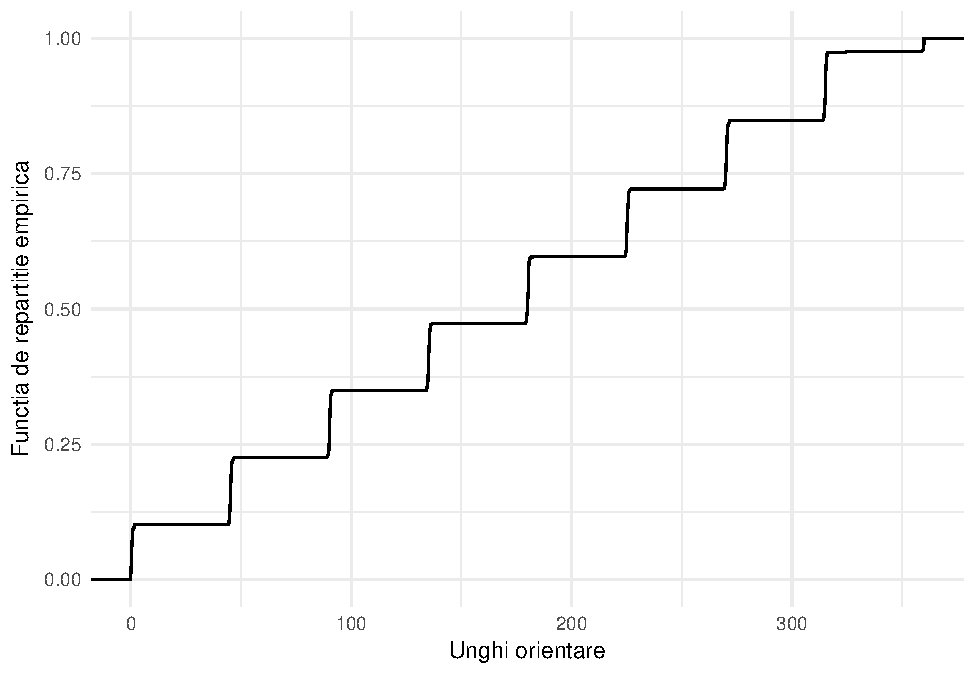
\includegraphics[width=0.7\linewidth]{Lab_Suplimentar_IPS_files/figure-latex/unnamed-chunk-16-1} \end{center}

ceea ce arată că observațiile sunt aglomerate în jurul celor 8 valori de
orientare. Următoarea funcție permite transformarea unghiurilor din
setul de date în unghiurile corespunzătoare orientăriilor celor mai
apropiate (e.g. \(47.5\) se duce în \(45\) și \(358.2\) se duce în
\(0\))

\begin{Shaded}
\begin{Highlighting}[]
\NormalTok{roundOrientation =}\StringTok{ }\ControlFlowTok{function}\NormalTok{(angles)\{}
\NormalTok{  refs =}\StringTok{ }\KeywordTok{seq}\NormalTok{(}\DecValTok{0}\NormalTok{,}\DecValTok{360}\NormalTok{, }\DataTypeTok{by =} \DecValTok{45}\NormalTok{)}
\NormalTok{  q =}\StringTok{ }\KeywordTok{sapply}\NormalTok{(angles, }\ControlFlowTok{function}\NormalTok{(x)\{}
        \KeywordTok{which.min}\NormalTok{(}\KeywordTok{abs}\NormalTok{(x}\OperatorTok{-}\NormalTok{refs))}
\NormalTok{      \})}\CommentTok{# indicii minimului }
\NormalTok{  a =}\StringTok{ }\KeywordTok{c}\NormalTok{(refs[}\DecValTok{1}\OperatorTok{:}\DecValTok{8}\NormalTok{], }\DecValTok{0}\NormalTok{)}\CommentTok{# schimba 360 in 0 }
  \KeywordTok{return}\NormalTok{(a[q])}
\NormalTok{\}}
\end{Highlighting}
\end{Shaded}

Schimbând orientările obținem rezultatul așteptat

\begin{Shaded}
\begin{Highlighting}[]
\NormalTok{offline}\OperatorTok{$}\NormalTok{angle =}\StringTok{ }\KeywordTok{roundOrientation}\NormalTok{(offline}\OperatorTok{$}\NormalTok{orientation)}
\end{Highlighting}
\end{Shaded}

\begin{center}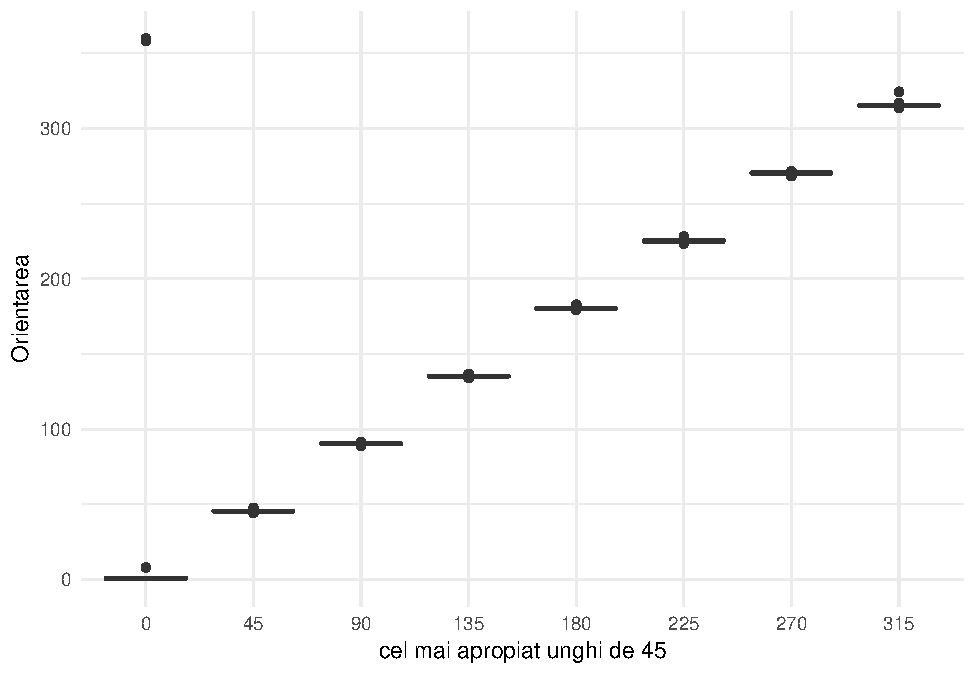
\includegraphics[width=0.7\linewidth]{Lab_Suplimentar_IPS_files/figure-latex/unnamed-chunk-19-1} \end{center}

\subsection{Să explorăm adresele MAC
emitente}\label{sa-exploram-adresele-mac-emitente}

Dacă ne uităm la datele sumarizate ale adreselor MAC emitente (ale
punctelor de acces) și ale frecvenței canalelor de emisie am putea
concluziona că există o bijecție între acestea:

\begin{verbatim}
                mac               channel      
 00:0f:a3:39:e1:c0:145862   2462000000:189774  
 00:0f:a3:39:dd:cd:145619   2437000000:152124  
 00:14:bf:b1:97:8a:132962   2412000000:145619  
 00:14:bf:3b:c7:c6:126529   2432000000:126529  
 00:14:bf:b1:97:90:122315   2427000000:122315  
 00:14:bf:b1:97:8d:121325   2442000000:121325  
 (Other)          :183831   (Other)   :120757  
\end{verbatim}

Dacă ne uităm la câte observații din fiecare adresă MAC avem, obținem că
sunt trei adrese cu un număr foarte mic de observații în comparație cu
celelalte ceea ce implică că aceste device-uri nu au fost aria de test
(poate au provenit de la un alt etaj) sau nu au fost active pe toată
durata testului.

\begin{Shaded}
\begin{Highlighting}[]
\KeywordTok{table}\NormalTok{(offline}\OperatorTok{$}\NormalTok{mac)}

\DecValTok{00}\OperatorTok{:}\DecValTok{04}\OperatorTok{:}\NormalTok{0e}\OperatorTok{:}\NormalTok{5c}\OperatorTok{:}\DecValTok{23}\OperatorTok{:}\NormalTok{fc }\DecValTok{00}\OperatorTok{:}\NormalTok{0f}\OperatorTok{:}\NormalTok{a3}\OperatorTok{:}\DecValTok{39}\OperatorTok{:}\NormalTok{dd}\OperatorTok{:}\NormalTok{cd }\DecValTok{00}\OperatorTok{:}\NormalTok{0f}\OperatorTok{:}\NormalTok{a3}\OperatorTok{:}\DecValTok{39}\OperatorTok{:}\NormalTok{e0}\OperatorTok{:}\NormalTok{4b }\DecValTok{00}\OperatorTok{:}\NormalTok{0f}\OperatorTok{:}\NormalTok{a3}\OperatorTok{:}\DecValTok{39}\OperatorTok{:}\NormalTok{e1}\OperatorTok{:}\NormalTok{c0 }
              \DecValTok{418}            \DecValTok{145619}             \DecValTok{43508}            \DecValTok{145862} 
\DecValTok{00}\OperatorTok{:}\NormalTok{0f}\OperatorTok{:}\NormalTok{a3}\OperatorTok{:}\DecValTok{39}\OperatorTok{:}\NormalTok{e2}\OperatorTok{:}\DecValTok{10} \DecValTok{00}\OperatorTok{:}\DecValTok{14}\OperatorTok{:}\NormalTok{bf}\OperatorTok{:}\NormalTok{3b}\OperatorTok{:}\NormalTok{c7}\OperatorTok{:}\NormalTok{c6 }\DecValTok{00}\OperatorTok{:}\DecValTok{14}\OperatorTok{:}\NormalTok{bf}\OperatorTok{:}\NormalTok{b1}\OperatorTok{:}\DecValTok{97}\OperatorTok{:}\DecValTok{81} \DecValTok{00}\OperatorTok{:}\DecValTok{14}\OperatorTok{:}\NormalTok{bf}\OperatorTok{:}\NormalTok{b1}\OperatorTok{:}\DecValTok{97}\OperatorTok{:}\NormalTok{8a }
            \DecValTok{19162}            \DecValTok{126529}            \DecValTok{120339}            \DecValTok{132962} 
\DecValTok{00}\OperatorTok{:}\DecValTok{14}\OperatorTok{:}\NormalTok{bf}\OperatorTok{:}\NormalTok{b1}\OperatorTok{:}\DecValTok{97}\OperatorTok{:}\NormalTok{8d }\DecValTok{00}\OperatorTok{:}\DecValTok{14}\OperatorTok{:}\NormalTok{bf}\OperatorTok{:}\NormalTok{b1}\OperatorTok{:}\DecValTok{97}\OperatorTok{:}\DecValTok{90} \DecValTok{00}\OperatorTok{:}\DecValTok{30}\OperatorTok{:}\NormalTok{bd}\OperatorTok{:}\NormalTok{f8}\OperatorTok{:}\NormalTok{7f}\OperatorTok{:}\NormalTok{c5 }\DecValTok{00}\OperatorTok{:}\NormalTok{e0}\OperatorTok{:}\DecValTok{63}\OperatorTok{:}\DecValTok{82}\OperatorTok{:}\NormalTok{8b}\OperatorTok{:}\NormalTok{a9 }
           \DecValTok{121325}            \DecValTok{122315}               \DecValTok{301}               \DecValTok{103} 
\end{Highlighting}
\end{Shaded}

Conform documentației setului de date știm că punctele de acces consistă
din 5 routere Linksys/Cisco și un router Lancom L-54g. Accesând pagina
\url{http://coffer.com/mac_find/} găsim că adresele care încep cu
\texttt{00:14:bf} aparțin producătorului Linksys/Cisco dar nu găsim o
corespondență cu routerul Lancom L-54g și prin urmare vom păstra primele
7 adrese după numărul de observații.

\begin{Shaded}
\begin{Highlighting}[]
\NormalTok{subMacs =}\StringTok{ }\KeywordTok{names}\NormalTok{(}\KeywordTok{sort}\NormalTok{(}\KeywordTok{table}\NormalTok{(offline}\OperatorTok{$}\NormalTok{mac), }\DataTypeTok{decreasing =} \OtherTok{TRUE}\NormalTok{))[}\DecValTok{1}\OperatorTok{:}\DecValTok{7}\NormalTok{]}

\CommentTok{# stergem observatiile canu nu se MAC-ul corespunzator}
\NormalTok{offline =}\StringTok{ }\NormalTok{offline[offline}\OperatorTok{$}\NormalTok{mac }\OperatorTok\StringTok{ }\NormalTok{subMacs, ]}

\CommentTok{# verificam daca avem corespondenta bijectiva}
\KeywordTok{table}\NormalTok{(offline[}\KeywordTok{c}\NormalTok{(}\StringTok{"mac"}\NormalTok{, }\StringTok{"channel"}\NormalTok{)])}
\NormalTok{                   channel}
\NormalTok{mac                 }\DecValTok{2412000000} \DecValTok{2422000000} \DecValTok{2427000000} \DecValTok{2432000000} \DecValTok{2437000000}
  \DecValTok{00}\OperatorTok{:}\NormalTok{0f}\OperatorTok{:}\NormalTok{a3}\OperatorTok{:}\DecValTok{39}\OperatorTok{:}\NormalTok{dd}\OperatorTok{:}\NormalTok{cd     }\DecValTok{145619}          \DecValTok{0}          \DecValTok{0}          \DecValTok{0}          \DecValTok{0}
  \DecValTok{00}\OperatorTok{:}\NormalTok{0f}\OperatorTok{:}\NormalTok{a3}\OperatorTok{:}\DecValTok{39}\OperatorTok{:}\NormalTok{e1}\OperatorTok{:}\NormalTok{c0          }\DecValTok{0}          \DecValTok{0}          \DecValTok{0}          \DecValTok{0}          \DecValTok{0}
  \DecValTok{00}\OperatorTok{:}\DecValTok{14}\OperatorTok{:}\NormalTok{bf}\OperatorTok{:}\NormalTok{3b}\OperatorTok{:}\NormalTok{c7}\OperatorTok{:}\NormalTok{c6          }\DecValTok{0}          \DecValTok{0}          \DecValTok{0}     \DecValTok{126529}          \DecValTok{0}
  \DecValTok{00}\OperatorTok{:}\DecValTok{14}\OperatorTok{:}\NormalTok{bf}\OperatorTok{:}\NormalTok{b1}\OperatorTok{:}\DecValTok{97}\OperatorTok{:}\DecValTok{81}          \DecValTok{0}     \DecValTok{120339}          \DecValTok{0}          \DecValTok{0}          \DecValTok{0}
  \DecValTok{00}\OperatorTok{:}\DecValTok{14}\OperatorTok{:}\NormalTok{bf}\OperatorTok{:}\NormalTok{b1}\OperatorTok{:}\DecValTok{97}\OperatorTok{:}\NormalTok{8a          }\DecValTok{0}          \DecValTok{0}          \DecValTok{0}          \DecValTok{0}     \DecValTok{132962}
  \DecValTok{00}\OperatorTok{:}\DecValTok{14}\OperatorTok{:}\NormalTok{bf}\OperatorTok{:}\NormalTok{b1}\OperatorTok{:}\DecValTok{97}\OperatorTok{:}\NormalTok{8d          }\DecValTok{0}          \DecValTok{0}          \DecValTok{0}          \DecValTok{0}          \DecValTok{0}
  \DecValTok{00}\OperatorTok{:}\DecValTok{14}\OperatorTok{:}\NormalTok{bf}\OperatorTok{:}\NormalTok{b1}\OperatorTok{:}\DecValTok{97}\OperatorTok{:}\DecValTok{90}          \DecValTok{0}          \DecValTok{0}     \DecValTok{122315}          \DecValTok{0}          \DecValTok{0}
\NormalTok{                   channel}
\NormalTok{mac                 }\DecValTok{2442000000} \DecValTok{2462000000}
  \DecValTok{00}\OperatorTok{:}\NormalTok{0f}\OperatorTok{:}\NormalTok{a3}\OperatorTok{:}\DecValTok{39}\OperatorTok{:}\NormalTok{dd}\OperatorTok{:}\NormalTok{cd          }\DecValTok{0}          \DecValTok{0}
  \DecValTok{00}\OperatorTok{:}\NormalTok{0f}\OperatorTok{:}\NormalTok{a3}\OperatorTok{:}\DecValTok{39}\OperatorTok{:}\NormalTok{e1}\OperatorTok{:}\NormalTok{c0          }\DecValTok{0}     \DecValTok{145862}
  \DecValTok{00}\OperatorTok{:}\DecValTok{14}\OperatorTok{:}\NormalTok{bf}\OperatorTok{:}\NormalTok{3b}\OperatorTok{:}\NormalTok{c7}\OperatorTok{:}\NormalTok{c6          }\DecValTok{0}          \DecValTok{0}
  \DecValTok{00}\OperatorTok{:}\DecValTok{14}\OperatorTok{:}\NormalTok{bf}\OperatorTok{:}\NormalTok{b1}\OperatorTok{:}\DecValTok{97}\OperatorTok{:}\DecValTok{81}          \DecValTok{0}          \DecValTok{0}
  \DecValTok{00}\OperatorTok{:}\DecValTok{14}\OperatorTok{:}\NormalTok{bf}\OperatorTok{:}\NormalTok{b1}\OperatorTok{:}\DecValTok{97}\OperatorTok{:}\NormalTok{8a          }\DecValTok{0}          \DecValTok{0}
  \DecValTok{00}\OperatorTok{:}\DecValTok{14}\OperatorTok{:}\NormalTok{bf}\OperatorTok{:}\NormalTok{b1}\OperatorTok{:}\DecValTok{97}\OperatorTok{:}\NormalTok{8d     }\DecValTok{121325}          \DecValTok{0}
  \DecValTok{00}\OperatorTok{:}\DecValTok{14}\OperatorTok{:}\NormalTok{bf}\OperatorTok{:}\NormalTok{b1}\OperatorTok{:}\DecValTok{97}\OperatorTok{:}\DecValTok{90}          \DecValTok{0}          \DecValTok{0}
\end{Highlighting}
\end{Shaded}

Cum avem o corespondență bijectivă între adresele MAC emitente și
frecvența canalelor de emisie putem elimina variabila \texttt{channel}
din setul de date:

\begin{Shaded}
\begin{Highlighting}[]
\CommentTok{# stergem variabila channel}
\NormalTok{offline =}\StringTok{ }\NormalTok{offline[, }\KeywordTok{names}\NormalTok{(offline)}\OperatorTok{!=}\StringTok{"channel"}\NormalTok{]}
\end{Highlighting}
\end{Shaded}

\subsection{Să explorăm poziția device-ului
mobil}\label{sa-exploram-pozitia-device-ului-mobil}

Investigăm care sunt locațiile diferite în care s-au înregistrat datele
și pentru aceasta apelăm funcția \texttt{by()}.

\begin{Shaded}
\begin{Highlighting}[]
\CommentTok{# functia by() verifica toate pereichile posibile}
\CommentTok{# aplica o functie la un data.frame impartiti dupa diverse categorii}
\NormalTok{locDF =}\StringTok{ }\KeywordTok{with}\NormalTok{(offline, }\KeywordTok{by}\NormalTok{(offline, }\KeywordTok{list}\NormalTok{(posX, posY), }
                         \ControlFlowTok{function}\NormalTok{(x) x))}
\KeywordTok{length}\NormalTok{(locDF) }\CommentTok{# marimea listei}
\NormalTok{[}\DecValTok{1}\NormalTok{] }\DecValTok{476}
\end{Highlighting}
\end{Shaded}

Conform documentației ne așteptăm să avem \(166\) de locații dar găsim
că avem 476, diferența reiese din faptul că multe din pozițiile
rezultate aplicând funcția \texttt{by()} sunt nule, mai exact avem

\begin{Shaded}
\begin{Highlighting}[]
\KeywordTok{sum}\NormalTok{(}\KeywordTok{sapply}\NormalTok{(locDF, is.null))}
\NormalTok{[}\DecValTok{1}\NormalTok{] }\DecValTok{310}

\CommentTok{# eliminam elementele nule}
\NormalTok{locDF =}\StringTok{ }\NormalTok{locDF[}\OperatorTok{!}\KeywordTok{sapply}\NormalTok{(locDF, is.null)]}
\end{Highlighting}
\end{Shaded}

Pentru a determina câte observații avem pentru fiecare locație în parte
și a reprezenta grafic aceste date avem:

\begin{Shaded}
\begin{Highlighting}[]
\CommentTok{# pastram si pozitia}
\NormalTok{locCounts =}\StringTok{ }\KeywordTok{sapply}\NormalTok{(locDF, }\ControlFlowTok{function}\NormalTok{(df)\{}
  \CommentTok{# fiecare element din locDF este un data.frame cu 8 coloane }
  \KeywordTok{c}\NormalTok{(df[}\DecValTok{1}\NormalTok{, }\KeywordTok{c}\NormalTok{(}\StringTok{"posX"}\NormalTok{,}\StringTok{"posY"}\NormalTok{)], }\DataTypeTok{count =} \KeywordTok{nrow}\NormalTok{(df))}
\NormalTok{\})}

\NormalTok{locCounts[, }\DecValTok{1}\OperatorTok{:}\DecValTok{8}\NormalTok{]}
\NormalTok{      [,}\DecValTok{1}\NormalTok{] [,}\DecValTok{2}\NormalTok{] [,}\DecValTok{3}\NormalTok{] [,}\DecValTok{4}\NormalTok{] [,}\DecValTok{5}\NormalTok{] [,}\DecValTok{6}\NormalTok{] [,}\DecValTok{7}\NormalTok{] [,}\DecValTok{8}\NormalTok{]}
\NormalTok{posX  }\DecValTok{0}    \DecValTok{1}    \DecValTok{2}    \DecValTok{0}    \DecValTok{1}    \DecValTok{2}    \DecValTok{0}    \DecValTok{1}   
\NormalTok{posY  }\DecValTok{0}    \DecValTok{0}    \DecValTok{0}    \DecValTok{1}    \DecValTok{1}    \DecValTok{1}    \DecValTok{2}    \DecValTok{2}   
\NormalTok{count }\DecValTok{5505} \DecValTok{5505} \DecValTok{5506} \DecValTok{5524} \DecValTok{5543} \DecValTok{5558} \DecValTok{5503} \DecValTok{5564}

\CommentTok{# pentru grafic }
\NormalTok{locCounts =}\StringTok{ }\KeywordTok{t}\NormalTok{(locCounts) }\CommentTok{# transpunem }
\end{Highlighting}
\end{Shaded}

\begin{verbatim}
Graficul cu coordonatele locatiilor
\end{verbatim}

\begin{center}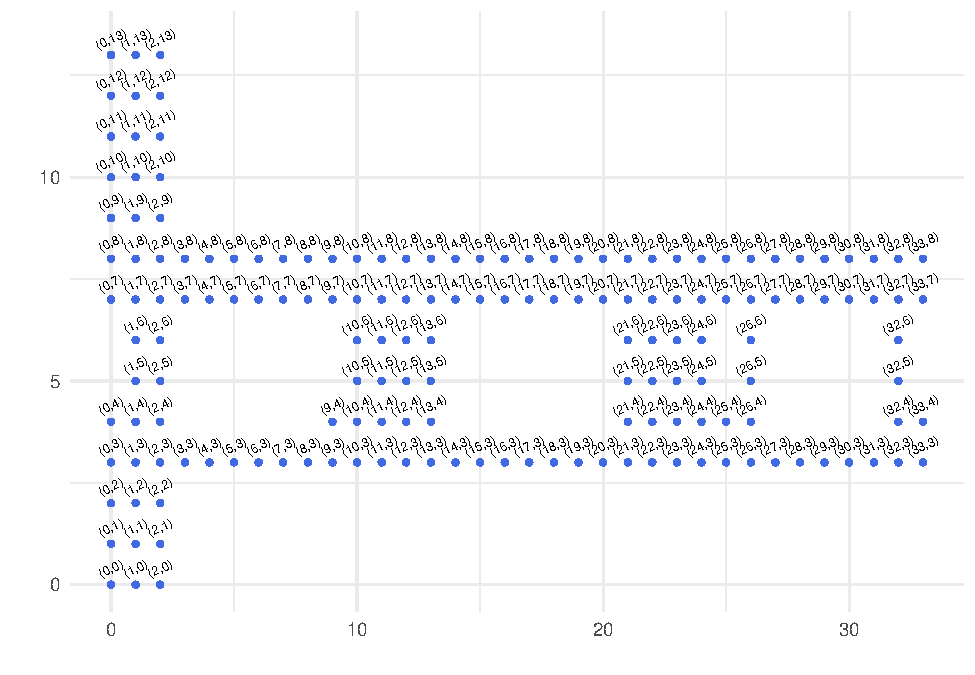
\includegraphics[width=0.8\linewidth]{Lab_Suplimentar_IPS_files/figure-latex/unnamed-chunk-27-1} \end{center}

\begin{verbatim}
Graficul cu numarul de observatii din fiecare locatie
\end{verbatim}

\begin{center}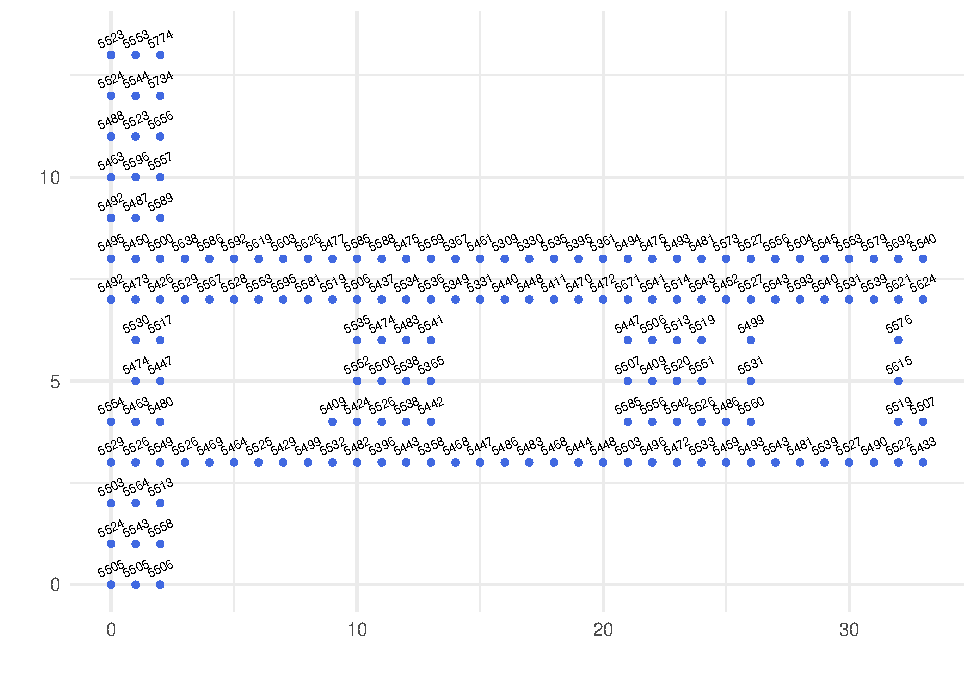
\includegraphics[width=0.8\linewidth]{Lab_Suplimentar_IPS_files/figure-latex/unnamed-chunk-28-1} \end{center}

Pentru reproductibilitate, sumarizăm toate operațiile efectuate până
acum într-o singură funcție \texttt{readData()}:

\begin{Shaded}
\begin{Highlighting}[]
\CommentTok{# Corpul functiei readData()}
\CommentTok{#----------------------------}

\NormalTok{readData =}\StringTok{ }
\StringTok{  }\ControlFlowTok{function}\NormalTok{(}\DataTypeTok{filename =} \StringTok{'lab_IPS_data/offline.final.trace.txt'}\NormalTok{, }
                   \DataTypeTok{subMacs =} \KeywordTok{c}\NormalTok{(}\StringTok{"00:0f:a3:39:e1:c0"}\NormalTok{, }
                               \StringTok{"00:0f:a3:39:dd:cd"}\NormalTok{, }
                               \StringTok{"00:14:bf:b1:97:8a"}\NormalTok{,}
                               \StringTok{"00:14:bf:3b:c7:c6"}\NormalTok{, }
                               \StringTok{"00:14:bf:b1:97:90"}\NormalTok{, }
                               \StringTok{"00:14:bf:b1:97:8d"}\NormalTok{,}
                               \StringTok{"00:14:bf:b1:97:81"}\NormalTok{))}
\NormalTok{  \{}
    \CommentTok{# functia care citeste si curata datele  }
    
\NormalTok{    doc =}\StringTok{ }\KeywordTok{readLines}\NormalTok{(filename)}\CommentTok{# citeste data }
\NormalTok{    doc =}\StringTok{ }\NormalTok{doc[}\KeywordTok{substr}\NormalTok{(doc,}\DecValTok{1}\NormalTok{,}\DecValTok{1}\NormalTok{)}\OperatorTok{!=}\StringTok{"#"}\NormalTok{]}\CommentTok{# sterge comment-urile }
    
\NormalTok{    tmp =}\StringTok{ }\KeywordTok{lapply}\NormalTok{(doc, processLine) }\CommentTok{# proceseaza documentul}
\NormalTok{    offline =}\StringTok{ }\KeywordTok{as.data.frame}\NormalTok{(}\KeywordTok{do.call}\NormalTok{(}\StringTok{"rbind"}\NormalTok{, tmp), }
                            \DataTypeTok{stringsAsFactors =} \OtherTok{FALSE}\NormalTok{)}\CommentTok{# in data.frame}
    
    \CommentTok{# numele variabilelor  }
    \KeywordTok{names}\NormalTok{(offline) =}\StringTok{ }\KeywordTok{c}\NormalTok{(}\StringTok{"time"}\NormalTok{,}\StringTok{"scanMac"}\NormalTok{, }\StringTok{"posX"}\NormalTok{, }\StringTok{"posY"}\NormalTok{, }
                       \StringTok{"posZ"}\NormalTok{, }\StringTok{"orientation"}\NormalTok{, }\StringTok{"mac"}\NormalTok{, }
                       \StringTok{"signal"}\NormalTok{, }\StringTok{"channel"}\NormalTok{, }\StringTok{"type"}\NormalTok{)}
    
    \CommentTok{# pastram semnale de la punctele de acces}
\NormalTok{    offline =}\StringTok{ }\NormalTok{offline[ offline}\OperatorTok{$}\NormalTok{type }\OperatorTok{==}\StringTok{ "3"}\NormalTok{, ]}
    
    \CommentTok{# eliminam var scanMac, posZ, channel, si type - }
    \CommentTok{#contin informatie redundanta}
\NormalTok{    dropVars =}\StringTok{ }\KeywordTok{c}\NormalTok{(}\StringTok{"scanMac"}\NormalTok{, }\StringTok{"posZ"}\NormalTok{, }\StringTok{"channel"}\NormalTok{, }\StringTok{"type"}\NormalTok{)}
\NormalTok{    offline =}\StringTok{ }\NormalTok{offline[ , }\OperatorTok{!}\NormalTok{( }\KeywordTok{names}\NormalTok{(offline) }\OperatorTok\StringTok{ }\NormalTok{dropVars ) ]}
    
    \CommentTok{# eliminam punctele de acces care nu prezinta interes}
\NormalTok{    offline =}\StringTok{ }\NormalTok{offline[ offline}\OperatorTok{$}\NormalTok{mac }\OperatorTok\StringTok{ }\NormalTok{subMacs, ]}
    
    \CommentTok{# transform variabilele in numeric }
\NormalTok{    numVars =}\StringTok{ }\KeywordTok{c}\NormalTok{(}\StringTok{"time"}\NormalTok{, }\StringTok{"posX"}\NormalTok{, }\StringTok{"posY"}\NormalTok{, }\StringTok{"orientation"}\NormalTok{, }\StringTok{"signal"}\NormalTok{)}
\NormalTok{    offline[numVars] =}\StringTok{ }\KeywordTok{lapply}\NormalTok{(offline[numVars], as.numeric)}
    
    \CommentTok{# pastram timpul raw}
\NormalTok{    offline}\OperatorTok{$}\NormalTok{rawTime =}\StringTok{ }\NormalTok{offline}\OperatorTok{$}\NormalTok{time}
\NormalTok{    offline}\OperatorTok{$}\NormalTok{time =}\StringTok{ }\NormalTok{offline}\OperatorTok{$}\NormalTok{time}\OperatorTok{/}\DecValTok{1000} \CommentTok{# ms in s}
    \KeywordTok{class}\NormalTok{(offline}\OperatorTok{$}\NormalTok{time) =}\StringTok{ }\KeywordTok{c}\NormalTok{(}\StringTok{"POSIXt"}\NormalTok{, }\StringTok{"POSIXct"}\NormalTok{)}
    
    \CommentTok{# rotunjim orientarile la 45 }
\NormalTok{    offline}\OperatorTok{$}\NormalTok{angle =}\StringTok{ }\KeywordTok{roundOrientation}\NormalTok{(offline}\OperatorTok{$}\NormalTok{orientation)}
    
    \KeywordTok{return}\NormalTok{(offline)}
    
    \CommentTok{# fct de procesare }
\NormalTok{    processLine =}\StringTok{ }\ControlFlowTok{function}\NormalTok{(x)\{}
      \CommentTok{# x este linia documentului }
      \CommentTok{# luam in considerare liniile mai scurte - cele care au mai }
      \CommentTok{# putin de 10 variabile (nu avem observatii de semnal)}
\NormalTok{      tokens =}\StringTok{ }\KeywordTok{strsplit}\NormalTok{(x, }\StringTok{"[;=,]"}\NormalTok{)[[}\DecValTok{1}\NormalTok{]]}
      \CommentTok{# pt obs care au 10 obs}
     
      \ControlFlowTok{if}\NormalTok{ (}\KeywordTok{length}\NormalTok{(tokens) }\OperatorTok{==}\StringTok{ }\DecValTok{10}\NormalTok{)\{}
        \KeywordTok{return}\NormalTok{(}\OtherTok{NULL}\NormalTok{)}
\NormalTok{      \}}
      
\NormalTok{      tmp =}\StringTok{ }\KeywordTok{matrix}\NormalTok{(tokens[}\OperatorTok{-}\NormalTok{(}\DecValTok{1}\OperatorTok{:}\DecValTok{10}\NormalTok{)], }\DataTypeTok{ncol =} \DecValTok{4}\NormalTok{, }\DataTypeTok{byrow =} \OtherTok{TRUE}\NormalTok{)}
      \KeywordTok{cbind}\NormalTok{(}\KeywordTok{matrix}\NormalTok{(tokens[}\KeywordTok{c}\NormalTok{(}\DecValTok{2}\NormalTok{,}\DecValTok{4}\NormalTok{,}\DecValTok{6}\OperatorTok{:}\DecValTok{8}\NormalTok{, }\DecValTok{10}\NormalTok{)], }\DataTypeTok{nrow =} \KeywordTok{nrow}\NormalTok{(tmp), }
                   \DataTypeTok{ncol =} \DecValTok{6}\NormalTok{, }\DataTypeTok{byrow =} \OtherTok{TRUE}\NormalTok{),tmp)}
\NormalTok{    \}}
    
    \CommentTok{# Functia de rotunjire a orientarilor }
\NormalTok{    roundOrientation =}\StringTok{ }\ControlFlowTok{function}\NormalTok{(angles)\{}
\NormalTok{      refs =}\StringTok{ }\KeywordTok{seq}\NormalTok{(}\DecValTok{0}\NormalTok{,}\DecValTok{360}\NormalTok{, }\DataTypeTok{by =} \DecValTok{45}\NormalTok{)}
\NormalTok{      q =}\StringTok{ }\KeywordTok{sapply}\NormalTok{(angles, }\ControlFlowTok{function}\NormalTok{(x)\{}
        \KeywordTok{which.min}\NormalTok{(}\KeywordTok{abs}\NormalTok{(x}\OperatorTok{-}\NormalTok{refs))}
\NormalTok{      \})}
\NormalTok{      a =}\StringTok{ }\KeywordTok{c}\NormalTok{(refs[}\DecValTok{1}\OperatorTok{:}\DecValTok{8}\NormalTok{], }\DecValTok{0}\NormalTok{)}\CommentTok{# 360 -> 0 }
      \KeywordTok{return}\NormalTok{(a[q])}
\NormalTok{    \}}
\NormalTok{  \}}
\end{Highlighting}
\end{Shaded}

Apelăm funcția

\begin{Shaded}
\begin{Highlighting}[]
\NormalTok{offline =}\StringTok{ }\KeywordTok{readData}\NormalTok{()}
\end{Highlighting}
\end{Shaded}

\section{Analiza intensității
semnalului}\label{analiza-intensitatii-semnalului}

În această secțiune ne propunem să investigăm care este comportamentul
variabilei intensitatea semnalului și să investigăm cum locația,
orientarea și punctul de acces poate influența repartiția intensității
semnalului.

\subsection{Repartiția intensității
semnalului}\label{repartitia-intensitatii-semnalului}

Ne propunem să comparăm cum este repartizată intensitatea semnalului în
funcție de diferite unghiuri de orientare și diferite puncte de acces.
Fixând o locație (e.g. \((x,y)=(22,4)\)) ne uităm cum variază
intensitatea semnalului odată cu schimbarea orientării:

\begin{center}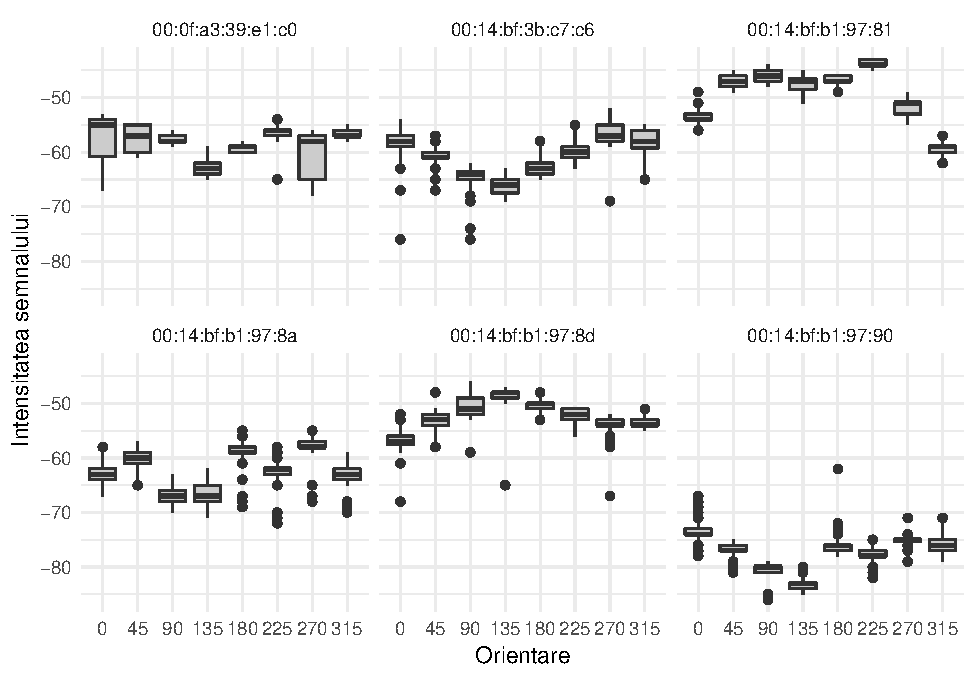
\includegraphics[width=0.8\linewidth]{Lab_Suplimentar_IPS_files/figure-latex/unnamed-chunk-31-1} \end{center}

Să ne reamintim că intensitatea semnalului se măsoară în valori negative
cu valori mici de tipul \(-98\) însemnând semnale slabe și valori mar de
tipul \(-25\) însemnând intensitate puternică. Repartiția intensității
semnalului pentru locația centrală \((x,y)=(12,5)\) în funcție de
fiecare orientare și adresă MAC este

\begin{center}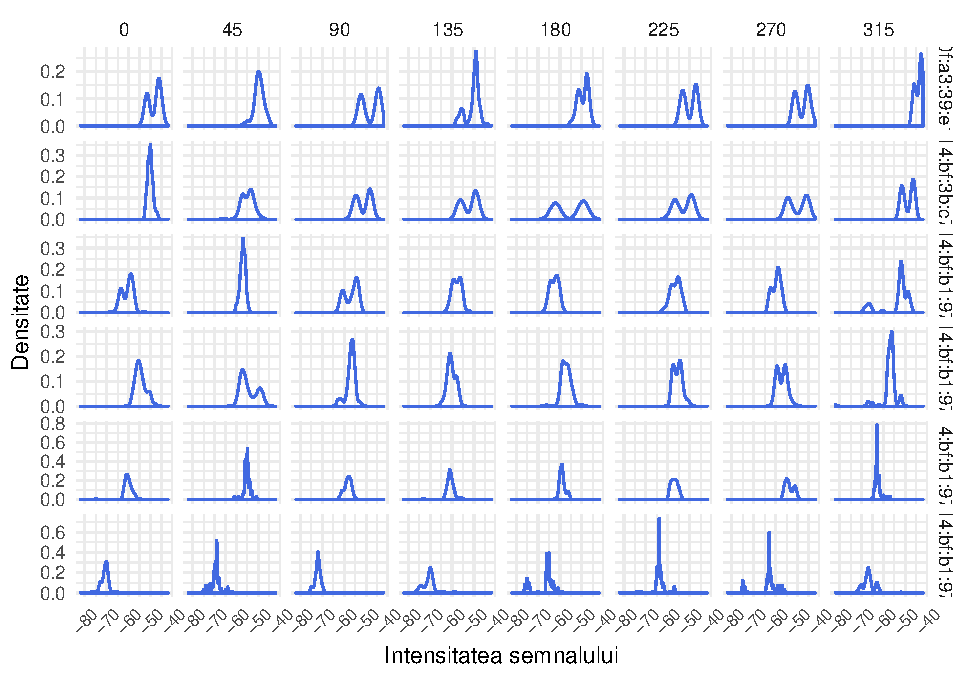
\includegraphics[width=1\linewidth]{Lab_Suplimentar_IPS_files/figure-latex/unnamed-chunk-32-1} \end{center}

Dacă am vrea să investigăm repartiția semnalului după toate cele 166 de
poziții, 8 orientări și 6 puncte de acces ar trebui să facem mii de
grafice și cum acest lucru este practic imposibil putem să sumarizăm
datele așa încât pentru fiecare pereche locație-orientare-punct de acces
să avem o valoare medie, mediană, o abatere standard și un interval
între cuartile IQR.

Începem prin a crea o nouă variabilă care conține toate perechile de
puncte \((x,y)\) și apoi creăm o listă de data.frame-uri pentru fiecare
combinație \((x,y)\), unghi și punct de acces:

\begin{Shaded}
\begin{Highlighting}[]
\NormalTok{offline}\OperatorTok{$}\NormalTok{posXY =}\StringTok{ }\KeywordTok{paste}\NormalTok{(offline}\OperatorTok{$}\NormalTok{posX, offline}\OperatorTok{$}\NormalTok{posY, }\DataTypeTok{sep =} \StringTok{"-"}\NormalTok{)}

\NormalTok{byLocAngleAP =}\StringTok{ }\KeywordTok{with}\NormalTok{(offline, }
                    \KeywordTok{by}\NormalTok{(offline, }\KeywordTok{list}\NormalTok{(posXY, angle, mac), }
                       \ControlFlowTok{function}\NormalTok{(x) x))}
\KeywordTok{length}\NormalTok{(byLocAngleAP) }\CommentTok{# cate data.frame-uri avem 166*8*7}
\NormalTok{[}\DecValTok{1}\NormalTok{] }\DecValTok{9296}
\end{Highlighting}
\end{Shaded}

și continuăm prin calculul statisticilor de sumarizare

\begin{Shaded}
\begin{Highlighting}[]
\NormalTok{signalSummary =}\StringTok{ }\KeywordTok{lapply}\NormalTok{(byLocAngleAP, }\ControlFlowTok{function}\NormalTok{(oneLoc)\{}
  \CommentTok{# creaza o data.frame care are aceleasi campuri ca cea originala}
\NormalTok{  ans =}\StringTok{ }\NormalTok{oneLoc[}\DecValTok{1}\NormalTok{, ] }
\NormalTok{  ans}\OperatorTok{$}\NormalTok{medSignal =}\StringTok{ }\KeywordTok{median}\NormalTok{(oneLoc}\OperatorTok{$}\NormalTok{signal)}
\NormalTok{  ans}\OperatorTok{$}\NormalTok{avgSignal =}\StringTok{ }\KeywordTok{mean}\NormalTok{(oneLoc}\OperatorTok{$}\NormalTok{signal)}
\NormalTok{  ans}\OperatorTok{$}\NormalTok{num =}\StringTok{ }\KeywordTok{length}\NormalTok{(oneLoc}\OperatorTok{$}\NormalTok{signal)}
\NormalTok{  ans}\OperatorTok{$}\NormalTok{sdSignal =}\StringTok{ }\KeywordTok{sd}\NormalTok{(oneLoc}\OperatorTok{$}\NormalTok{signal)}
\NormalTok{  ans}\OperatorTok{$}\NormalTok{irqSignal =}\StringTok{ }\KeywordTok{IQR}\NormalTok{(oneLoc}\OperatorTok{$}\NormalTok{signal)}
  \KeywordTok{return}\NormalTok{(ans)}
\NormalTok{\})}

\CommentTok{# cream un data.frame din variabilele sumarizate}
\NormalTok{offlineSummary =}\StringTok{ }\KeywordTok{do.call}\NormalTok{(}\StringTok{"rbind"}\NormalTok{, signalSummary) }
\end{Highlighting}
\end{Shaded}

Ne uităm dacă abaterile standard variază în funcție de intensitatea
medie a semnalului recepționat și constatăm că semnalele slabe au o
abatere standard mai mică și aceasta crește odată cu creșterea
intensității semnalului.

\begin{center}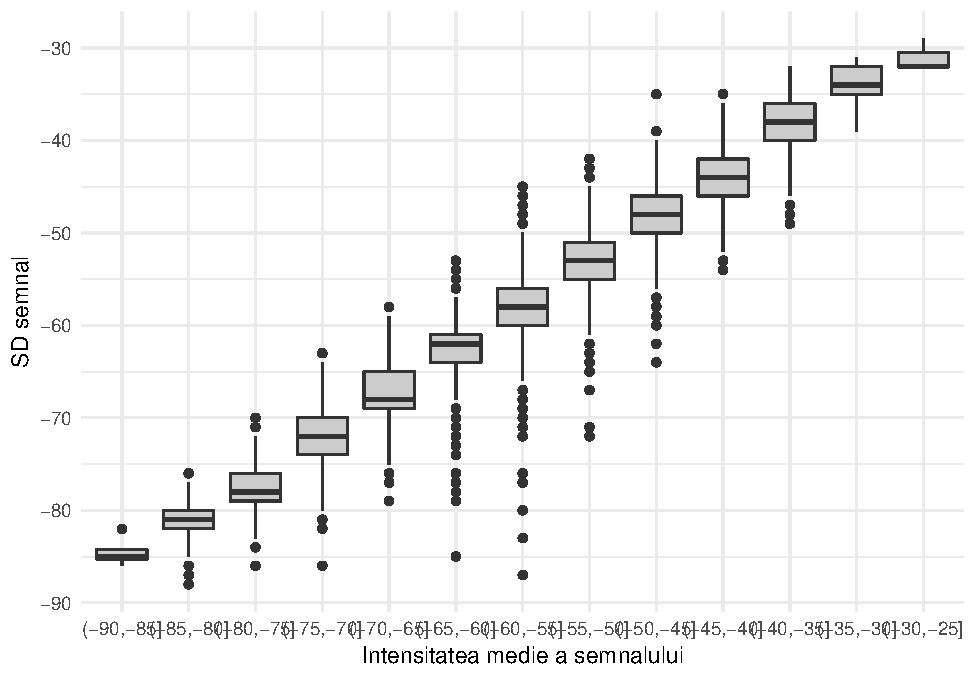
\includegraphics[width=0.7\linewidth]{Lab_Suplimentar_IPS_files/figure-latex/unnamed-chunk-35-1} \end{center}

\subsection{Cum influențează distanța semnalul
?}\label{cum-influenteaza-distanta-semnalul}

Pentru a vedea cum este influențat semnalul în funcție de distanță vom
trasa o hartă topografică (un heat map) folosind pachetul
\texttt{fields} care o folosește o metodă de tip spline pentru a potrivi
(fit) o suprafață în locațiile date după valorile intensității
semnalului recepționat. Funcția \texttt{Tps()} (Thin plate spline
regression) necesită pentru fiecare pereche de puncte \((x,y)\) o unică
valoare \(z\) și prin urmare vom folosi setul de date
\emph{offlineSummary}:

\begin{Shaded}
\begin{Highlighting}[]
\CommentTok{# functia care traseaza pentru o adresa MAC si un unghi }
\CommentTok{# heat map-ul necesar}
\NormalTok{surfaceSS =}\StringTok{ }\ControlFlowTok{function}\NormalTok{(data, mac, }\DataTypeTok{angle =} \DecValTok{45}\NormalTok{, ...)\{}
  \KeywordTok{require}\NormalTok{(fields) }\CommentTok{# avem nevoie de acest pachet}
  
  \CommentTok{# subsectionam data}
\NormalTok{  oneAPAngle =}\StringTok{ }\NormalTok{data[data}\OperatorTok{$}\NormalTok{mac }\OperatorTok{==}\StringTok{ }\NormalTok{mac }\OperatorTok{&}\StringTok{ }\NormalTok{data}\OperatorTok{$}\NormalTok{angle }\OperatorTok{==}\StringTok{ }\NormalTok{angle, ] }
  
  \CommentTok{# construim suprafata prin regresie spline}
\NormalTok{  smoothSS =}\StringTok{ }\KeywordTok{Tps}\NormalTok{(oneAPAngle[, }\KeywordTok{c}\NormalTok{(}\StringTok{"posX"}\NormalTok{,}\StringTok{"posY"}\NormalTok{)], oneAPAngle}\OperatorTok{$}\NormalTok{avgSignal)}
  
  \CommentTok{# transforma functia fitata intr-o suprafata plotabila}
\NormalTok{  vizSmooth =}\StringTok{ }\KeywordTok{predictSurface}\NormalTok{(smoothSS)}
  \KeywordTok{plot.surface}\NormalTok{(vizSmooth, }\DataTypeTok{type =} \StringTok{"C"}\NormalTok{, }
               \DataTypeTok{xlab =} \StringTok{""}\NormalTok{, }\DataTypeTok{ylab =} \StringTok{""}\NormalTok{, }\DataTypeTok{xaxt =} \StringTok{"n"}\NormalTok{, }\DataTypeTok{yaxt =} \StringTok{"n"}\NormalTok{, }
               \DataTypeTok{bty =} \StringTok{"n"}\NormalTok{, ...)}
  
  \KeywordTok{points}\NormalTok{(oneAPAngle}\OperatorTok{$}\NormalTok{posX, oneAPAngle}\OperatorTok{$}\NormalTok{posY, }\DataTypeTok{pch=}\DecValTok{19}\NormalTok{, }\DataTypeTok{cex =} \FloatTok{0.5}\NormalTok{)}
\NormalTok{\}}
\end{Highlighting}
\end{Shaded}

\begin{verbatim}
Graficul pentru adresa MAC  00:0f:a3:39:e1:c0 
\end{verbatim}

\begin{center}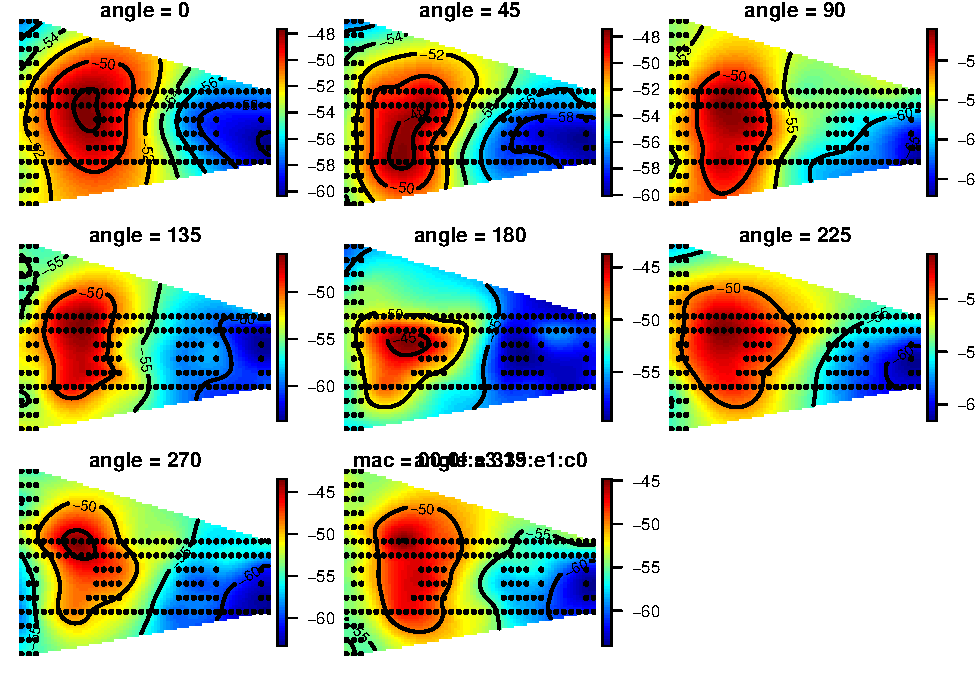
\includegraphics[width=0.7\linewidth]{Lab_Suplimentar_IPS_files/figure-latex/unnamed-chunk-37-1} \end{center}

\begin{verbatim}
Graficul pentru adresa MAC  00:0f:a3:39:dd:cd 
\end{verbatim}

\begin{center}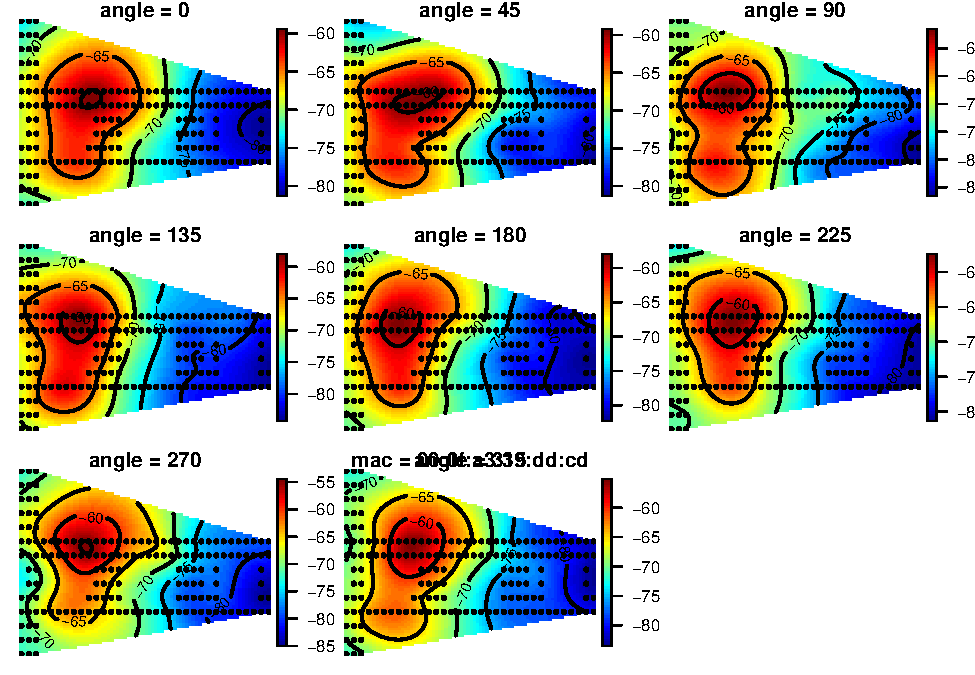
\includegraphics[width=0.7\linewidth]{Lab_Suplimentar_IPS_files/figure-latex/unnamed-chunk-37-2} \end{center}

\begin{verbatim}
Graficul pentru adresa MAC  00:14:bf:b1:97:8a 
\end{verbatim}

\begin{center}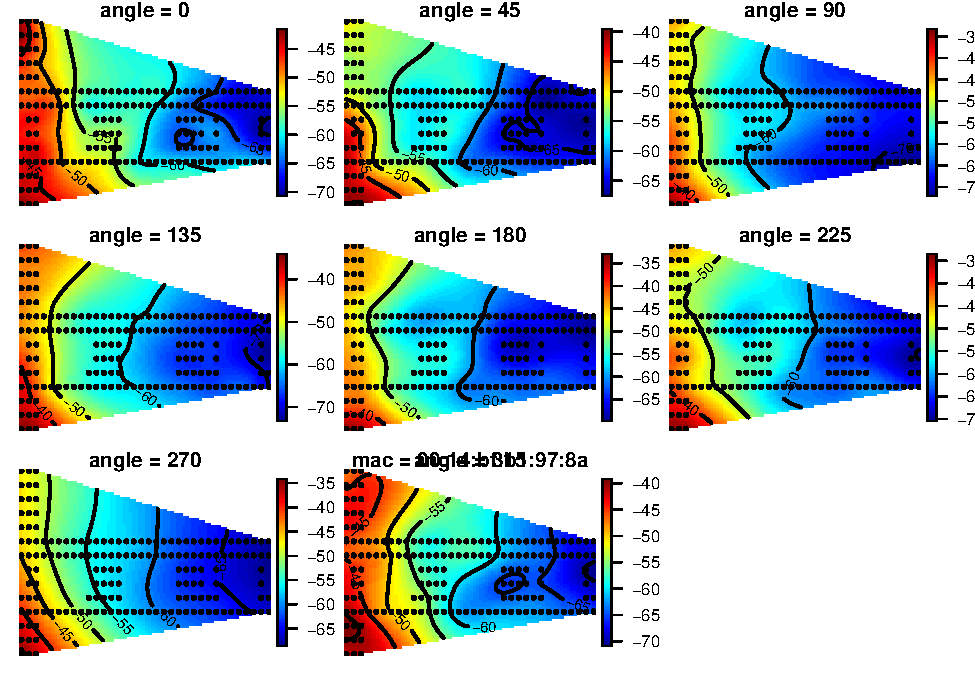
\includegraphics[width=0.7\linewidth]{Lab_Suplimentar_IPS_files/figure-latex/unnamed-chunk-37-3} \end{center}

\begin{verbatim}
Graficul pentru adresa MAC  00:14:bf:3b:c7:c6 
\end{verbatim}

\begin{center}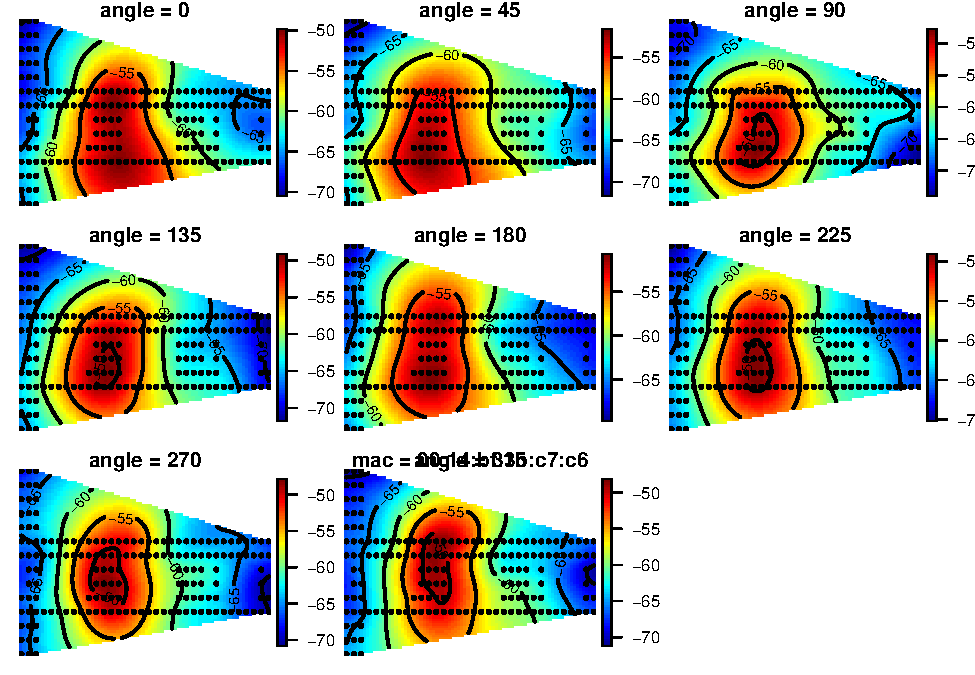
\includegraphics[width=0.7\linewidth]{Lab_Suplimentar_IPS_files/figure-latex/unnamed-chunk-37-4} \end{center}

\begin{verbatim}
Graficul pentru adresa MAC  00:14:bf:b1:97:90 
\end{verbatim}

\begin{center}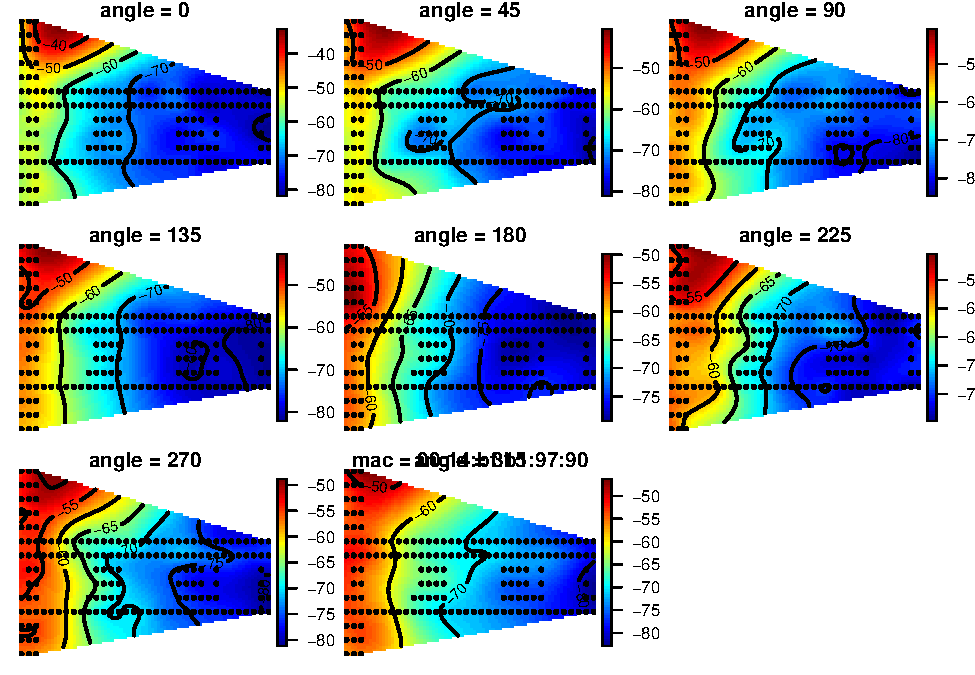
\includegraphics[width=0.7\linewidth]{Lab_Suplimentar_IPS_files/figure-latex/unnamed-chunk-37-5} \end{center}

\begin{verbatim}
Graficul pentru adresa MAC  00:14:bf:b1:97:8d 
\end{verbatim}

\begin{center}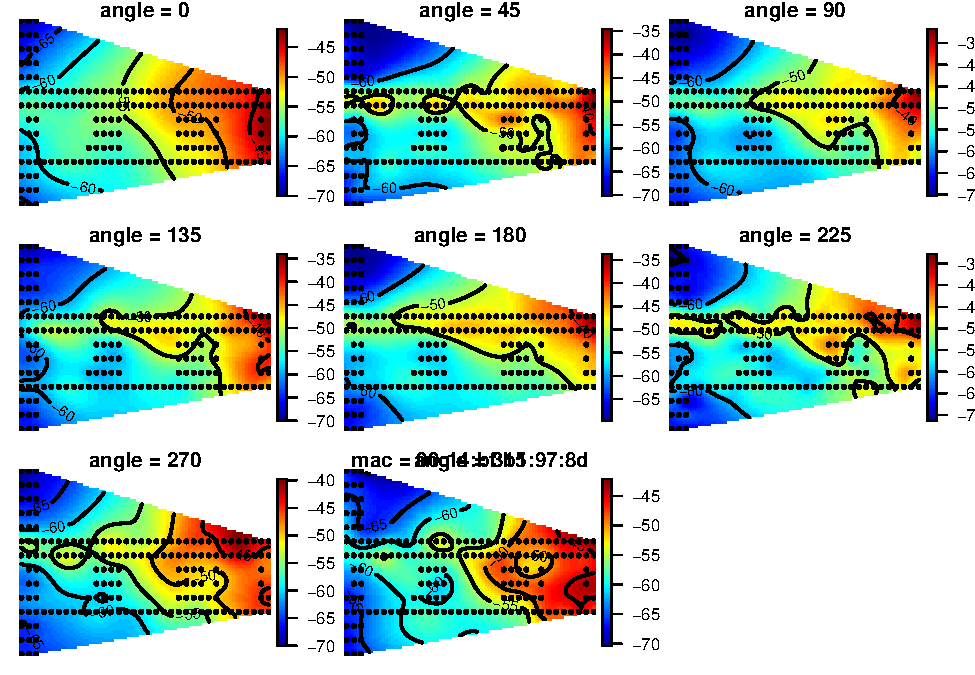
\includegraphics[width=0.7\linewidth]{Lab_Suplimentar_IPS_files/figure-latex/unnamed-chunk-37-6} \end{center}

\begin{verbatim}
Graficul pentru adresa MAC  00:14:bf:b1:97:81 
\end{verbatim}

\begin{center}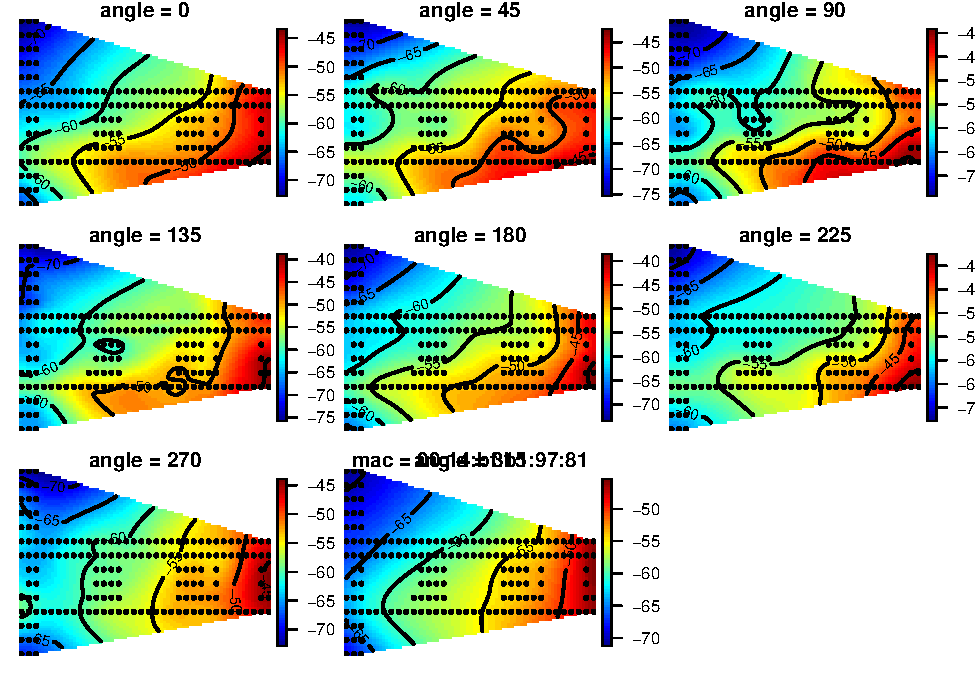
\includegraphics[width=0.7\linewidth]{Lab_Suplimentar_IPS_files/figure-latex/unnamed-chunk-37-7} \end{center}

Graficele de mai sus ne spun și unde se află locațiile punctelor de
acces pe plan. Putem să creăm o matrice cu pozițiile și numele celor 6
puncte de acces:

\begin{Shaded}
\begin{Highlighting}[]
\NormalTok{AP =}\StringTok{ }\KeywordTok{matrix}\NormalTok{(}\KeywordTok{c}\NormalTok{(}\FloatTok{7.5}\NormalTok{, }\FloatTok{6.3}\NormalTok{, }\FloatTok{2.5}\NormalTok{, }\OperatorTok{-}\NormalTok{.}\DecValTok{8}\NormalTok{, }\FloatTok{12.8}\NormalTok{, }\OperatorTok{-}\FloatTok{2.8}\NormalTok{, }
              \DecValTok{1}\NormalTok{, }\DecValTok{14}\NormalTok{, }\FloatTok{33.5}\NormalTok{, }\FloatTok{9.3}\NormalTok{, }\FloatTok{33.5}\NormalTok{, }\FloatTok{2.8}\NormalTok{), }
            \DataTypeTok{ncol =} \DecValTok{2}\NormalTok{, }\DataTypeTok{byrow =} \OtherTok{TRUE}\NormalTok{, }
            \DataTypeTok{dimnames =} \KeywordTok{list}\NormalTok{(subMacs[}\OperatorTok{-}\DecValTok{2}\NormalTok{], }\KeywordTok{c}\NormalTok{(}\StringTok{"x"}\NormalTok{, }\StringTok{"y"}\NormalTok{)))}
\NormalTok{AP}
\NormalTok{                     x    y}
\DecValTok{00}\OperatorTok{:}\NormalTok{0f}\OperatorTok{:}\NormalTok{a3}\OperatorTok{:}\DecValTok{39}\OperatorTok{:}\NormalTok{e1}\OperatorTok{:}\NormalTok{c0  }\FloatTok{7.5}  \FloatTok{6.3}
\DecValTok{00}\OperatorTok{:}\DecValTok{14}\OperatorTok{:}\NormalTok{bf}\OperatorTok{:}\NormalTok{b1}\OperatorTok{:}\DecValTok{97}\OperatorTok{:}\NormalTok{8a  }\FloatTok{2.5} \OperatorTok{-}\FloatTok{0.8}
\DecValTok{00}\OperatorTok{:}\DecValTok{14}\OperatorTok{:}\NormalTok{bf}\OperatorTok{:}\NormalTok{3b}\OperatorTok{:}\NormalTok{c7}\OperatorTok{:}\NormalTok{c6 }\FloatTok{12.8} \OperatorTok{-}\FloatTok{2.8}
\DecValTok{00}\OperatorTok{:}\DecValTok{14}\OperatorTok{:}\NormalTok{bf}\OperatorTok{:}\NormalTok{b1}\OperatorTok{:}\DecValTok{97}\OperatorTok{:}\DecValTok{90}  \FloatTok{1.0} \FloatTok{14.0}
\DecValTok{00}\OperatorTok{:}\DecValTok{14}\OperatorTok{:}\NormalTok{bf}\OperatorTok{:}\NormalTok{b1}\OperatorTok{:}\DecValTok{97}\OperatorTok{:}\NormalTok{8d }\FloatTok{33.5}  \FloatTok{9.3}
\DecValTok{00}\OperatorTok{:}\DecValTok{14}\OperatorTok{:}\NormalTok{bf}\OperatorTok{:}\NormalTok{b1}\OperatorTok{:}\DecValTok{97}\OperatorTok{:}\DecValTok{81} \FloatTok{33.5}  \FloatTok{2.8}
\end{Highlighting}
\end{Shaded}

\begin{center}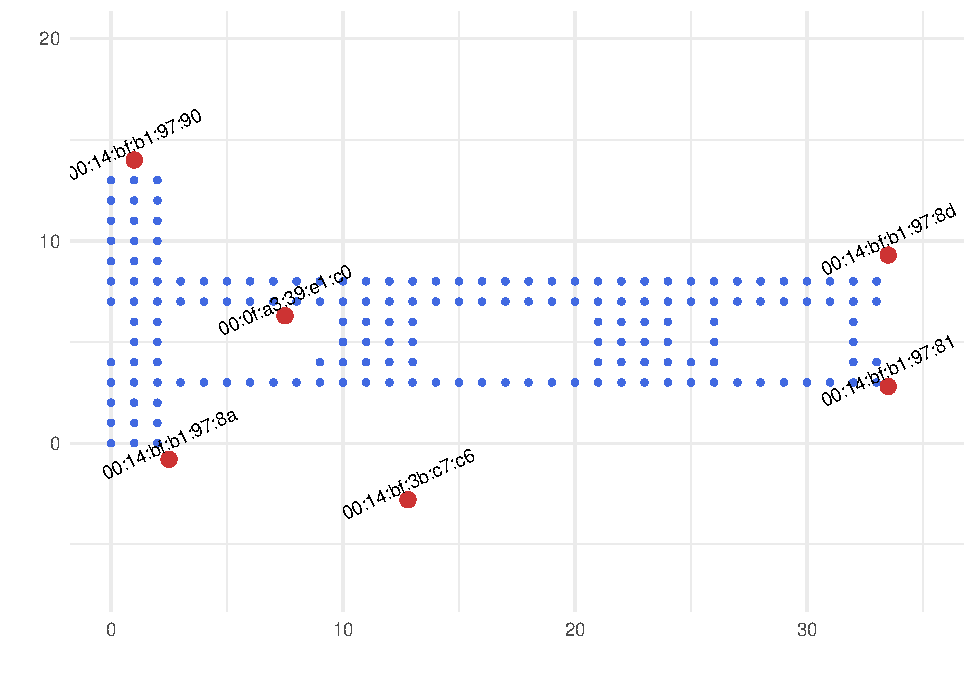
\includegraphics[width=0.7\linewidth]{Lab_Suplimentar_IPS_files/figure-latex/unnamed-chunk-39-1} \end{center}

Pentru a vedea ce relație există între intensitatea semnalului și
distanța de la punctul de acces putem să calculăm distanțele de la
locația device-ului până la punctele de acces (distanța Euclidiană)

\begin{Shaded}
\begin{Highlighting}[]
\NormalTok{offlineSummary =}\StringTok{ }\KeywordTok{subset}\NormalTok{(offlineSummary, mac }\OperatorTok{!=}\StringTok{ }\NormalTok{subMacs[}\DecValTok{2}\NormalTok{])}

\CommentTok{# calculam diferenta de pozitie x si y dintre }
\CommentTok{# locatie si punctul de acces}
\NormalTok{diffs =}\StringTok{ }\NormalTok{offlineSummary[, }\KeywordTok{c}\NormalTok{(}\StringTok{"posX"}\NormalTok{, }\StringTok{"posY"}\NormalTok{)] }\OperatorTok{-}\StringTok{ }
\StringTok{  }\NormalTok{AP[offlineSummary}\OperatorTok{$}\NormalTok{mac, ]}

\CommentTok{# dist Euclidiana}
\NormalTok{offlineSummary}\OperatorTok{$}\NormalTok{dist =}\StringTok{ }\KeywordTok{sqrt}\NormalTok{(diffs[ ,}\DecValTok{1}\NormalTok{]}\OperatorTok{^}\DecValTok{2} \OperatorTok{+}\StringTok{ }\NormalTok{diffs[, }\DecValTok{2}\NormalTok{]}\OperatorTok{^}\DecValTok{2}\NormalTok{)}
\end{Highlighting}
\end{Shaded}

\begin{center}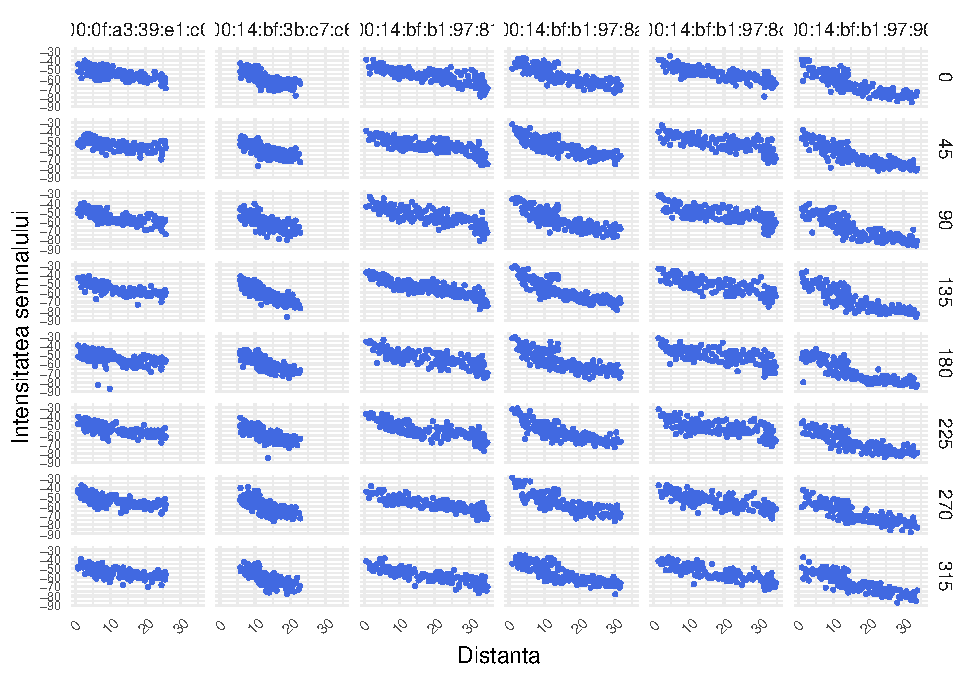
\includegraphics[width=1\linewidth]{Lab_Suplimentar_IPS_files/figure-latex/unnamed-chunk-41-1} \end{center}

\section{Metodă de prezicere a locației bazată pe cei mai apropiați
vecini}\label{metoda-de-prezicere-a-locatiei-bazata-pe-cei-mai-apropiati-vecini}

Pentru a putea estima locația unei noi observații pe baza intensității
semnalului dintre un device mobil aflat în acea locație și câteva puncte
de acces fixate, vom folosi metoda celor mai apropiați \(k\) vecini
(\(k\)-nearest neighbors sau \(k-NN\)). Idea din spatele acestei metode
este următoarea: avem un set de date de antrenament (training data) în
care intensitatea semnalului către cele 6 puncte de acces fixe este
măsurată din diferite poziții cunoscute din interiorul clădirii în care
se desfășoară experimentul; atunci când avem o observație nouă, ceea ce
înseamnă că avem un nou set de măsurători a intensității semnalului
efectuate din locația necunoscută către punctele de acces, găsim \(k\)
observații din setul de date de antrenament care sunt cele mai
\emph{similare} de noua observație. Prin \emph{similare} înțelegem că
intensitatea semnalelor înregistrate între punctele de acces și noua
observație a cărei locație este necunoscută este apropiată de
intensitatea semnalelor înregistrate între punctele de acces și cele
\(k\) observații. Estimăm poziția observației noi prin agregarea
poziției celor \(k\) observații din datele de antrenament.

Vom măsura distanța dintre două seturi de intensități de semnale cu
ajutorul metricii Euclidiene\footnote{Binențeles se pot alege și alte
  metrici pentru a calcula similaritatea dintre două observații,
  e.g.~metrica
  \href{https://en.wikipedia.org/wiki/Mahalanobis_distance}{Mahalanobis}
  sau
  \href{https://en.wikipedia.org/wiki/Minkowski_distance}{Minkowski},
  distanța Euclidiană este un caz particular de Minkowski (\(p=2\)).},
anume având date două observații \(o1\) și \(o2\), acestea sunt
caracterizate fiecare de un 6-tuplu de intensități de semnale
\((S_1^i,S_3^i, S_3^i,S_4^i, S_5^i, S_6^i)\), \(i\in\{1,2\}\) către cele
6 puncte de acces și

\[
  d_E(o1,o2) = \sqrt{(S_1^2-S_1^2)^2 + (S_2^2-S_2^2)^2 + (S_3^2-S_3^2)^2 + (S_4^2-S_4^2)^2 + (S_5^2-S_5^2)^2 + (S_6^2-S_6^2)^2}
\]

\subsection{Pregătirea setului de date
online}\label{pregatirea-setului-de-date-online}

Setul de date de test este setul de date \emph{online} (acestea sunt
noile observații a căror locație vrem să o estimăm). Vom folosi funcția
\texttt{readData()} pentru a preprocesa (curăța și aduce la forma dorită
pentru analiză) acest set de date.

\begin{Shaded}
\begin{Highlighting}[]
\CommentTok{# valorile adreselor mac pt cele 6 puncte de acces}
\NormalTok{macs =}\StringTok{ }\KeywordTok{unique}\NormalTok{(offlineSummary}\OperatorTok{$}\NormalTok{mac)}
\NormalTok{online =}\StringTok{ }\KeywordTok{readData}\NormalTok{(}\DataTypeTok{filename =} \StringTok{"lab_IPS_data/online.final.trace.txt"}\NormalTok{,}
                  \DataTypeTok{subMacs =}\NormalTok{ macs)}
\end{Highlighting}
\end{Shaded}

Pentru a ne face o impresie preliminară asupra acestui set de date, vrem
să ilustrăm câte observații avem pentru fiecare pereche \emph{locație -
unghi orientare}

\begin{Shaded}
\begin{Highlighting}[]
\CommentTok{# cream o noua variabila prin unirea perechii x-y}
\NormalTok{online}\OperatorTok{$}\NormalTok{posXY =}\StringTok{ }\KeywordTok{paste}\NormalTok{(online}\OperatorTok{$}\NormalTok{posX, online}\OperatorTok{$}\NormalTok{posY, }\DataTypeTok{sep =} \StringTok{"-"}\NormalTok{)}

\CommentTok{# cate noi locatii avem?}
\KeywordTok{length}\NormalTok{(}\KeywordTok{unique}\NormalTok{(online}\OperatorTok{$}\NormalTok{posXY))}
\NormalTok{[}\DecValTok{1}\NormalTok{] }\DecValTok{60}

\NormalTok{tabonlineXYA =}\StringTok{ }\KeywordTok{table}\NormalTok{(online}\OperatorTok{$}\NormalTok{posXY, online}\OperatorTok{$}\NormalTok{angle)}
\KeywordTok{head}\NormalTok{(tabonlineXYA, }\DecValTok{10}\NormalTok{)}
            
               \DecValTok{0}  \DecValTok{45}  \DecValTok{90} \DecValTok{135} \DecValTok{180} \DecValTok{225} \DecValTok{270} \DecValTok{315}
  \DecValTok{0}\OperatorTok{-}\FloatTok{0.05}       \DecValTok{0}   \DecValTok{0}   \DecValTok{0} \DecValTok{593}   \DecValTok{0}   \DecValTok{0}   \DecValTok{0}   \DecValTok{0}
  \FloatTok{0.15}\OperatorTok{-}\FloatTok{9.42}    \DecValTok{0}   \DecValTok{0} \DecValTok{606}   \DecValTok{0}   \DecValTok{0}   \DecValTok{0}   \DecValTok{0}   \DecValTok{0}
  \FloatTok{0.31}\OperatorTok{-}\FloatTok{11.09}   \DecValTok{0}   \DecValTok{0}   \DecValTok{0}   \DecValTok{0}   \DecValTok{0} \DecValTok{573}   \DecValTok{0}   \DecValTok{0}
  \FloatTok{0.47}\OperatorTok{-}\FloatTok{8.2}   \DecValTok{590}   \DecValTok{0}   \DecValTok{0}   \DecValTok{0}   \DecValTok{0}   \DecValTok{0}   \DecValTok{0}   \DecValTok{0}
  \FloatTok{0.78}\OperatorTok{-}\FloatTok{10.94} \DecValTok{586}   \DecValTok{0}   \DecValTok{0}   \DecValTok{0}   \DecValTok{0}   \DecValTok{0}   \DecValTok{0}   \DecValTok{0}
  \FloatTok{0.93}\OperatorTok{-}\FloatTok{11.69}   \DecValTok{0}   \DecValTok{0}   \DecValTok{0}   \DecValTok{0} \DecValTok{583}   \DecValTok{0}   \DecValTok{0}   \DecValTok{0}
  \FloatTok{1.08}\OperatorTok{-}\FloatTok{12.19}   \DecValTok{0}   \DecValTok{0}   \DecValTok{0}   \DecValTok{0}   \DecValTok{0} \DecValTok{630}   \DecValTok{0}   \DecValTok{0}
  \FloatTok{1.24}\OperatorTok{-}\FloatTok{3.93}    \DecValTok{0}   \DecValTok{0}   \DecValTok{0}   \DecValTok{0}   \DecValTok{0}   \DecValTok{0} \DecValTok{574}   \DecValTok{0}
  \FloatTok{1.39}\OperatorTok{-}\FloatTok{6.61}    \DecValTok{0}   \DecValTok{0}   \DecValTok{0} \DecValTok{595}   \DecValTok{0}   \DecValTok{0}   \DecValTok{0}   \DecValTok{0}
  \FloatTok{1.52}\OperatorTok{-}\FloatTok{9.32}  \DecValTok{583}   \DecValTok{0}   \DecValTok{0}   \DecValTok{0}   \DecValTok{0}   \DecValTok{0}   \DecValTok{0}   \DecValTok{0}
\end{Highlighting}
\end{Shaded}

Tabelul de mai sus ne arată că pentru fiecare locație au fost
înregistrate intensitățile semnalelor pentru o singură orientare și nu
pentru 8 orientări ca și în cazul setului de date \emph{offline}.

Vrem să organizăm datele \emph{online} pentru analiză într-un data.frame
care să conțină informații sumarizate pe câte o coloană pentru fiecare
dintre cele 6 puncte de acces în care să se înregistreze valoarea
intensității semnalului corespunzător (este diferit față de organizarea
datelor \emph{offline} întrucât în această situație știm în prealabil
câte punte de acces emit semnal - 6). Păstrăm în setul de date doar
acele informații care permit estimarea pozițiilor: poziția, orientarea
și intensitatea semnalului pentru fiecare din cele 6 puncte de acces.

\begin{Shaded}
\begin{Highlighting}[]
\CommentTok{# ce variabile pastram}
\NormalTok{keepVars =}\StringTok{ }\KeywordTok{c}\NormalTok{(}\StringTok{"posXY"}\NormalTok{, }\StringTok{"posX"}\NormalTok{, }\StringTok{"posY"}\NormalTok{, }\StringTok{"orientation"}\NormalTok{, }\StringTok{"angle"}\NormalTok{)}

\CommentTok{# sumarizam observatiile - dupa medie}
\NormalTok{byLoc =}\StringTok{ }\KeywordTok{with}\NormalTok{(online, }\KeywordTok{by}\NormalTok{(online, }\KeywordTok{list}\NormalTok{(posXY), }\ControlFlowTok{function}\NormalTok{(x) \{}
\NormalTok{  ans =}\StringTok{ }\NormalTok{x[}\DecValTok{1}\NormalTok{,keepVars]}
\NormalTok{  avgSS =}\StringTok{ }\KeywordTok{tapply}\NormalTok{(x}\OperatorTok{$}\NormalTok{signal, x}\OperatorTok{$}\NormalTok{mac, mean)}
\NormalTok{  y =}\StringTok{ }\KeywordTok{matrix}\NormalTok{(avgSS, }\DataTypeTok{nrow =} \DecValTok{1}\NormalTok{, }\DataTypeTok{ncol =} \DecValTok{6}\NormalTok{, }\DataTypeTok{dimnames =} \KeywordTok{list}\NormalTok{(ans}\OperatorTok{$}\NormalTok{posXY, }\KeywordTok{names}\NormalTok{(avgSS)))}
  \KeywordTok{cbind}\NormalTok{(ans, y)}
\NormalTok{\}))}

\CommentTok{# datele sumarizate}
\NormalTok{onlineSummary =}\StringTok{ }\KeywordTok{do.call}\NormalTok{(}\StringTok{"rbind"}\NormalTok{, byLoc)}


\KeywordTok{dim}\NormalTok{(onlineSummary)}
\NormalTok{[}\DecValTok{1}\NormalTok{] }\DecValTok{60} \DecValTok{11}
\KeywordTok{names}\NormalTok{(onlineSummary)}
\NormalTok{ [}\DecValTok{1}\NormalTok{] }\StringTok{"posXY"}             \StringTok{"posX"}              \StringTok{"posY"}             
\NormalTok{ [}\DecValTok{4}\NormalTok{] }\StringTok{"orientation"}       \StringTok{"angle"}             \StringTok{"00:0f:a3:39:e1:c0"}
\NormalTok{ [}\DecValTok{7}\NormalTok{] }\StringTok{"00:14:bf:3b:c7:c6"} \StringTok{"00:14:bf:b1:97:81"} \StringTok{"00:14:bf:b1:97:8a"}
\NormalTok{[}\DecValTok{10}\NormalTok{] }\StringTok{"00:14:bf:b1:97:8d"} \StringTok{"00:14:bf:b1:97:90"}
\end{Highlighting}
\end{Shaded}

Deoarece în modelul bazat pe cei mai apropiați vecini dorim să comparăm
observațiile noi cu cele din setul de date \emph{offline} în vederea
găsirii acelor observații care sunt cele mai apropiate în sensul
intensității semnalelor măsurate față de cele 6 puncte de acces, ar
trebui ca acestea din urmă să prezinte caracteristici similare cu cele
cu care le comparăm, de exemplu am vrea să comparăm observații care au
orientare similară cu cele noi. Pentru aceasta vom considera toate
observațiile care au orientarea într-un interval specificat. De exemplu
dacă dorim doar o orientare atunci alegem din setul de date
\emph{offline} doar pe acelea care au aceeași orientare (după rotunjire)
cu cea a noii observații (tot după rotunjire la unghi de 45 de grade).
Dacă în schimb dorim două orientări atunci le alegem orientările
(multiplii de 45 de grade) care mărginesc orientarea observației noi.

\begin{Shaded}
\begin{Highlighting}[]
\CommentTok{# pentru numarul de orientari m}
\NormalTok{m =}\StringTok{ }\DecValTok{3}

\CommentTok{# unghiul noii observatii}
\NormalTok{angleNewObs =}\StringTok{ }\DecValTok{230}

\CommentTok{# determinam cel mai apropiat unghi de 45}
\NormalTok{refs =}\StringTok{ }\KeywordTok{seq}\NormalTok{(}\DecValTok{0}\NormalTok{, }\DataTypeTok{by =} \DecValTok{45}\NormalTok{, }\DataTypeTok{length =} \DecValTok{8}\NormalTok{)}
\NormalTok{nearestAngle =}\StringTok{ }\KeywordTok{roundOrientation}\NormalTok{(angleNewObs)}

\CommentTok{# dupa cum m este par sau impar}
\ControlFlowTok{if}\NormalTok{ (m }\OperatorTok\StringTok{ }\DecValTok{2} \OperatorTok{==}\StringTok{ }\DecValTok{1}\NormalTok{)\{}
\NormalTok{  angles =}\StringTok{ }\KeywordTok{seq}\NormalTok{(}\OperatorTok{-}\DecValTok{45}\OperatorTok{*}\NormalTok{(m}\OperatorTok{-}\DecValTok{1}\NormalTok{)}\OperatorTok{/}\DecValTok{2}\NormalTok{, }\DecValTok{45}\OperatorTok{*}\NormalTok{(m}\OperatorTok{-}\DecValTok{1}\NormalTok{)}\OperatorTok{/}\DecValTok{2}\NormalTok{, }\DataTypeTok{length =}\NormalTok{ m)}
\NormalTok{\}}\ControlFlowTok{else}\NormalTok{\{}
\NormalTok{  m =}\StringTok{ }\NormalTok{m}\OperatorTok{+}\DecValTok{1}
\NormalTok{  angles =}\StringTok{ }\KeywordTok{seq}\NormalTok{(}\OperatorTok{-}\DecValTok{45}\OperatorTok{*}\NormalTok{(m}\OperatorTok{-}\DecValTok{1}\NormalTok{)}\OperatorTok{/}\DecValTok{2}\NormalTok{, }\DecValTok{45}\OperatorTok{*}\NormalTok{(m}\OperatorTok{-}\DecValTok{1}\NormalTok{)}\OperatorTok{/}\DecValTok{2}\NormalTok{, }\DataTypeTok{length =}\NormalTok{ m)}
  \ControlFlowTok{if}\NormalTok{ (}\KeywordTok{sign}\NormalTok{(angleNewObs }\OperatorTok{-}\StringTok{ }\NormalTok{nearestAngle)}\OperatorTok{>-}\DecValTok{1}\NormalTok{)\{}
\NormalTok{    angles =}\StringTok{ }\NormalTok{angles[}\OperatorTok{-}\DecValTok{1}\NormalTok{]}
\NormalTok{  \}}\ControlFlowTok{else}\NormalTok{\{}
\NormalTok{    angles =}\StringTok{ }\NormalTok{angles[}\OperatorTok{-}\NormalTok{m]}
\NormalTok{  \}}
\NormalTok{\}}
\CommentTok{# transformam unghiurile si le ajustam }
\CommentTok{# e.g. -45 -> 315 si 405 -> 45}
\NormalTok{angles =}\StringTok{ }\NormalTok{angles }\OperatorTok{+}\StringTok{ }\NormalTok{nearestAngle}
\NormalTok{angles[angles}\OperatorTok{<}\DecValTok{0}\NormalTok{] =}\StringTok{ }\NormalTok{angles[angles}\OperatorTok{<}\DecValTok{0}\NormalTok{] }\OperatorTok{+}\StringTok{ }\DecValTok{360}
\NormalTok{angles[angles}\OperatorTok{>}\DecValTok{360}\NormalTok{] =}\StringTok{ }\NormalTok{angles[angles}\OperatorTok{>}\DecValTok{360}\NormalTok{] }\OperatorTok{-}\StringTok{ }\DecValTok{360}

\CommentTok{# alegem observatiile cu unghiurile corespunzatoarea}
\NormalTok{offlineSubset =}\StringTok{ }\NormalTok{offlineSummary[offlineSummary}\OperatorTok{$}\NormalTok{angle }\OperatorTok\StringTok{ }\NormalTok{angles, ]}
\end{Highlighting}
\end{Shaded}

Transformăm setul de date ales (cel de antrenament) în același format cu
cel pentru datele de test \texttt{onlineSummary} cu ajutorul unei
funcții:

\begin{Shaded}
\begin{Highlighting}[]
\NormalTok{reshapeSS =}\StringTok{ }\ControlFlowTok{function}\NormalTok{(data, }\DataTypeTok{varSignal =} \StringTok{"signal"}\NormalTok{, }
                     \DataTypeTok{keepVars =} \KeywordTok{c}\NormalTok{(}\StringTok{"posXY"}\NormalTok{, }\StringTok{"posX"}\NormalTok{, }\StringTok{"posY"}\NormalTok{))\{}
\NormalTok{  byLocation =}\StringTok{ }\KeywordTok{with}\NormalTok{(data, }\KeywordTok{by}\NormalTok{(data, }\KeywordTok{list}\NormalTok{(posXY), }\ControlFlowTok{function}\NormalTok{(x)\{}
\NormalTok{    ans =}\StringTok{ }\NormalTok{x[}\DecValTok{1}\NormalTok{,keepVars]}
\NormalTok{    avgSS =}\StringTok{ }\KeywordTok{tapply}\NormalTok{(x[,varSignal], x}\OperatorTok{$}\NormalTok{mac, mean)}
\NormalTok{    y =}\StringTok{ }\KeywordTok{matrix}\NormalTok{(avgSS, }\DataTypeTok{nrow =} \DecValTok{1}\NormalTok{, }\DataTypeTok{ncol =} \DecValTok{6}\NormalTok{, }
               \DataTypeTok{dimnames =} \KeywordTok{list}\NormalTok{(ans}\OperatorTok{$}\NormalTok{posXY, }\KeywordTok{names}\NormalTok{(avgSS)))}
    \KeywordTok{cbind}\NormalTok{(ans, y)}
\NormalTok{  \}))}
\NormalTok{  newDataSS =}\StringTok{ }\KeywordTok{do.call}\NormalTok{(}\StringTok{"rbind"}\NormalTok{, byLocation)}
  \KeywordTok{return}\NormalTok{(newDataSS)}
\NormalTok{\}}

\CommentTok{# sumarizam setul de date de antrenament }
\NormalTok{trainSS =}\StringTok{ }\KeywordTok{reshapeSS}\NormalTok{(offlineSubset, }\DataTypeTok{varSignal =} \StringTok{"avgSignal"}\NormalTok{)}
\end{Highlighting}
\end{Shaded}

Creăm o funcție care să automatizeze acest proces: selecție de unghiuri
de orientare și transformare de date pentru antrenament. Funcția
\texttt{selectTrain()} calculează media intensității semnalelor ce
corespund la diferite orientări pentru a produce un singur 6-tuplu de
intensități de semnele pentru fiecare din cele 166 de locații.

\begin{Shaded}
\begin{Highlighting}[]
\CommentTok{# numim functia selectTrain()}
\NormalTok{selectTrain =}\StringTok{ }\ControlFlowTok{function}\NormalTok{(angleNewObs, }\DataTypeTok{signals =} \OtherTok{NULL}\NormalTok{, }\DataTypeTok{m =} \DecValTok{1}\NormalTok{)\{}
\NormalTok{  refs =}\StringTok{ }\KeywordTok{seq}\NormalTok{(}\DecValTok{0}\NormalTok{, }\DataTypeTok{by =} \DecValTok{45}\NormalTok{, }\DataTypeTok{length =} \DecValTok{8}\NormalTok{)}
\NormalTok{  nearestAngle =}\StringTok{ }\KeywordTok{roundOrientation}\NormalTok{(angleNewObs)}
  
  \ControlFlowTok{if}\NormalTok{ (m }\OperatorTok\StringTok{ }\DecValTok{2} \OperatorTok{==}\StringTok{ }\DecValTok{1}\NormalTok{)\{}
\NormalTok{    angles =}\StringTok{ }\KeywordTok{seq}\NormalTok{(}\OperatorTok{-}\DecValTok{45}\OperatorTok{*}\NormalTok{(m}\OperatorTok{-}\DecValTok{1}\NormalTok{)}\OperatorTok{/}\DecValTok{2}\NormalTok{, }\DecValTok{45}\OperatorTok{*}\NormalTok{(m}\OperatorTok{-}\DecValTok{1}\NormalTok{)}\OperatorTok{/}\DecValTok{2}\NormalTok{, }\DataTypeTok{length =}\NormalTok{ m)}
\NormalTok{  \}}\ControlFlowTok{else}\NormalTok{\{}
\NormalTok{    m =}\StringTok{ }\NormalTok{m}\OperatorTok{+}\DecValTok{1}
\NormalTok{    angles =}\StringTok{ }\KeywordTok{seq}\NormalTok{(}\OperatorTok{-}\DecValTok{45}\OperatorTok{*}\NormalTok{(m}\OperatorTok{-}\DecValTok{1}\NormalTok{)}\OperatorTok{/}\DecValTok{2}\NormalTok{, }\DecValTok{45}\OperatorTok{*}\NormalTok{(m}\OperatorTok{-}\DecValTok{1}\NormalTok{)}\OperatorTok{/}\DecValTok{2}\NormalTok{, }\DataTypeTok{length =}\NormalTok{ m)}
    \ControlFlowTok{if}\NormalTok{ (}\KeywordTok{sign}\NormalTok{(angleNewObs }\OperatorTok{-}\StringTok{ }\NormalTok{nearestAngle)}\OperatorTok{>-}\DecValTok{1}\NormalTok{)\{}
\NormalTok{      angles =}\StringTok{ }\NormalTok{angles[}\OperatorTok{-}\DecValTok{1}\NormalTok{]}
\NormalTok{    \}}\ControlFlowTok{else}\NormalTok{\{}
\NormalTok{      angles =}\StringTok{ }\NormalTok{angles[}\OperatorTok{-}\NormalTok{m]}
\NormalTok{    \}}
\NormalTok{  \}}
  \CommentTok{# transformam unghiurile si le ajustam }
  \CommentTok{# e.g. -45 -> 315 si 405 -> 45}
\NormalTok{  angles =}\StringTok{ }\NormalTok{angles }\OperatorTok{+}\StringTok{ }\NormalTok{nearestAngle}
\NormalTok{  angles[angles}\OperatorTok{<}\DecValTok{0}\NormalTok{] =}\StringTok{ }\NormalTok{angles[angles}\OperatorTok{<}\DecValTok{0}\NormalTok{] }\OperatorTok{+}\StringTok{ }\DecValTok{360}
\NormalTok{  angles[angles}\OperatorTok{>}\DecValTok{360}\NormalTok{] =}\StringTok{ }\NormalTok{angles[angles}\OperatorTok{>}\DecValTok{360}\NormalTok{] }\OperatorTok{-}\StringTok{ }\DecValTok{360}
\NormalTok{  angles =}\StringTok{ }\KeywordTok{sort}\NormalTok{(angles) }
  
\NormalTok{  offlineSubset =}\StringTok{ }\NormalTok{signals[signals}\OperatorTok{$}\NormalTok{angle }\OperatorTok\StringTok{ }\NormalTok{angles, ]}
  \KeywordTok{reshapeSS}\NormalTok{(offlineSubset, }\DataTypeTok{varSignal =} \StringTok{"avgSignal"}\NormalTok{)}
\NormalTok{\}}

\CommentTok{# testam pentru unghiul 130 si m = 3}
\NormalTok{train130 =}\StringTok{ }\KeywordTok{selectTrain}\NormalTok{(}\DecValTok{130}\NormalTok{, offlineSummary, }\DecValTok{3}\NormalTok{)}
\KeywordTok{head}\NormalTok{(train130)}
\NormalTok{     posXY posX posY }\DecValTok{00}\OperatorTok{:}\NormalTok{0f}\OperatorTok{:}\NormalTok{a3}\OperatorTok{:}\DecValTok{39}\OperatorTok{:}\NormalTok{e1}\OperatorTok{:}\NormalTok{c0 }\DecValTok{00}\OperatorTok{:}\DecValTok{14}\OperatorTok{:}\NormalTok{bf}\OperatorTok{:}\NormalTok{3b}\OperatorTok{:}\NormalTok{c7}\OperatorTok{:}\NormalTok{c6 }\DecValTok{00}\OperatorTok{:}\DecValTok{14}\OperatorTok{:}\NormalTok{bf}\OperatorTok{:}\NormalTok{b1}\OperatorTok{:}\DecValTok{97}\OperatorTok{:}\DecValTok{81}
\DecValTok{0}\OperatorTok{-}\DecValTok{0}    \DecValTok{0}\OperatorTok{-}\DecValTok{0}    \DecValTok{0}    \DecValTok{0}         \OperatorTok{-}\FloatTok{52.37243}         \OperatorTok{-}\FloatTok{66.13039}         \OperatorTok{-}\FloatTok{63.19262}
\DecValTok{0}\OperatorTok{-}\DecValTok{1}    \DecValTok{0}\OperatorTok{-}\DecValTok{1}    \DecValTok{0}    \DecValTok{1}         \OperatorTok{-}\FloatTok{52.98182}         \OperatorTok{-}\FloatTok{65.37177}         \OperatorTok{-}\FloatTok{63.72941}
\DecValTok{0}\OperatorTok{-}\DecValTok{10}  \DecValTok{0}\OperatorTok{-}\DecValTok{10}    \DecValTok{0}   \DecValTok{10}         \OperatorTok{-}\FloatTok{56.34184}         \OperatorTok{-}\FloatTok{65.67238}         \OperatorTok{-}\FloatTok{69.16041}
\DecValTok{0}\OperatorTok{-}\DecValTok{11}  \DecValTok{0}\OperatorTok{-}\DecValTok{11}    \DecValTok{0}   \DecValTok{11}         \OperatorTok{-}\FloatTok{54.73420}         \OperatorTok{-}\FloatTok{67.17593}         \OperatorTok{-}\FloatTok{70.34538}
\DecValTok{0}\OperatorTok{-}\DecValTok{12}  \DecValTok{0}\OperatorTok{-}\DecValTok{12}    \DecValTok{0}   \DecValTok{12}         \OperatorTok{-}\FloatTok{56.03030}         \OperatorTok{-}\FloatTok{70.46493}         \OperatorTok{-}\FloatTok{72.28758}
\DecValTok{0}\OperatorTok{-}\DecValTok{13}  \DecValTok{0}\OperatorTok{-}\DecValTok{13}    \DecValTok{0}   \DecValTok{13}         \OperatorTok{-}\FloatTok{54.55152}         \OperatorTok{-}\FloatTok{71.19211}         \OperatorTok{-}\FloatTok{72.58496}
     \DecValTok{00}\OperatorTok{:}\DecValTok{14}\OperatorTok{:}\NormalTok{bf}\OperatorTok{:}\NormalTok{b1}\OperatorTok{:}\DecValTok{97}\OperatorTok{:}\NormalTok{8a }\DecValTok{00}\OperatorTok{:}\DecValTok{14}\OperatorTok{:}\NormalTok{bf}\OperatorTok{:}\NormalTok{b1}\OperatorTok{:}\DecValTok{97}\OperatorTok{:}\NormalTok{8d }\DecValTok{00}\OperatorTok{:}\DecValTok{14}\OperatorTok{:}\NormalTok{bf}\OperatorTok{:}\NormalTok{b1}\OperatorTok{:}\DecValTok{97}\OperatorTok{:}\DecValTok{90}
\DecValTok{0}\OperatorTok{-}\DecValTok{0}          \OperatorTok{-}\FloatTok{35.58063}         \OperatorTok{-}\FloatTok{64.25411}         \OperatorTok{-}\FloatTok{55.33780}
\DecValTok{0}\OperatorTok{-}\DecValTok{1}          \OperatorTok{-}\FloatTok{39.37649}         \OperatorTok{-}\FloatTok{65.44867}         \OperatorTok{-}\FloatTok{59.15328}
\DecValTok{0}\OperatorTok{-}\DecValTok{10}         \OperatorTok{-}\FloatTok{44.71545}         \OperatorTok{-}\FloatTok{66.85781}         \OperatorTok{-}\FloatTok{50.45502}
\DecValTok{0}\OperatorTok{-}\DecValTok{11}         \OperatorTok{-}\FloatTok{48.34689}         \OperatorTok{-}\FloatTok{66.78383}         \OperatorTok{-}\FloatTok{54.93054}
\DecValTok{0}\OperatorTok{-}\DecValTok{12}         \OperatorTok{-}\FloatTok{45.17264}         \OperatorTok{-}\FloatTok{66.72696}         \OperatorTok{-}\FloatTok{50.49886}
\DecValTok{0}\OperatorTok{-}\DecValTok{13}         \OperatorTok{-}\FloatTok{43.32784}         \OperatorTok{-}\FloatTok{68.72616}         \OperatorTok{-}\FloatTok{54.48160}
\end{Highlighting}
\end{Shaded}

\subsection{Să găsim cei mai apropiați
vecini}\label{sa-gasim-cei-mai-apropiati-vecini}

În această secțiune construim funcția \texttt{findNN()} care permite
găsirea celor mai apropiați \(k\) vecini de noua observație din setul de
date de test. Funcția primește ca date de intrare un vector numeric de
lungime 6 ce corespunde intensității semnalelor pentru noua observație
și datele de antrenament rezultate din aplicarea funcției
\texttt{selectTrain()}. Ca date de ieșire funcția întoarce locațiile
observațiilor din setul de date de antrenament în funcție de apropierea
de observația nouă, de test.

\begin{Shaded}
\begin{Highlighting}[]
\CommentTok{# functia findNN}
\NormalTok{findNN =}\StringTok{ }\ControlFlowTok{function}\NormalTok{(newSignal, trainSubset)\{}
  \CommentTok{# aplicam functia x-newSignal liniilor }
\NormalTok{  diffs =}\StringTok{ }\KeywordTok{apply}\NormalTok{(trainSubset[, }\DecValTok{4}\OperatorTok{:}\DecValTok{9}\NormalTok{], }\DecValTok{1}\NormalTok{, }\ControlFlowTok{function}\NormalTok{(x) x}\OperatorTok{-}\NormalTok{newSignal)}
  
  \CommentTok{# aplicam functia coloanelor }
\NormalTok{  dists =}\StringTok{ }\KeywordTok{apply}\NormalTok{(diffs, }\DecValTok{2}\NormalTok{, }\ControlFlowTok{function}\NormalTok{(x) }\KeywordTok{sqrt}\NormalTok{(}\KeywordTok{sum}\NormalTok{(x}\OperatorTok{^}\DecValTok{2}\NormalTok{)))}
  
  \CommentTok{# ordonam observatiile}
\NormalTok{  closest =}\StringTok{ }\KeywordTok{order}\NormalTok{(dists)}
  
  \CommentTok{# intoarcem pozitiile obs ordonate}
  \KeywordTok{return}\NormalTok{(trainSubset[closest, }\DecValTok{1}\OperatorTok{:}\DecValTok{3}\NormalTok{])}
\NormalTok{\}}
\end{Highlighting}
\end{Shaded}

Estimam pozitiile noilor puncte cu ajutorul funcției \texttt{predXY()}
care calculează media aritmetică a locațiilor celor mai apropiate \(k\)
puncte (aici puteți să dați o metodă alternativă de calcul a
locațiilor):

\begin{Shaded}
\begin{Highlighting}[]
\CommentTok{# functia predXY}
\NormalTok{predXY =}\StringTok{ }\ControlFlowTok{function}\NormalTok{(newSignals, newAngles, trainData, }
                  \DataTypeTok{numAngles =} \DecValTok{1}\NormalTok{, }\DataTypeTok{k =} \DecValTok{3}\NormalTok{)\{}
  
\NormalTok{  closeXY =}\StringTok{ }\KeywordTok{list}\NormalTok{(}\DataTypeTok{length =} \KeywordTok{nrow}\NormalTok{(newSignals))}
  
  \ControlFlowTok{for}\NormalTok{ (i }\ControlFlowTok{in} \DecValTok{1}\OperatorTok{:}\KeywordTok{nrow}\NormalTok{(newSignals))\{}
\NormalTok{    trainSS =}\StringTok{ }\KeywordTok{selectTrain}\NormalTok{(newAngles[i], trainData, }\DataTypeTok{m =}\NormalTok{ numAngles)}
\NormalTok{    closeXY[[i]] =}\StringTok{ }\KeywordTok{findNN}\NormalTok{(}\DataTypeTok{newSignal =} \KeywordTok{as.numeric}\NormalTok{(newSignals[i,]), trainSS)}
\NormalTok{  \}}
  \CommentTok{# estimam locatia }
\NormalTok{  estXY =}\StringTok{ }\KeywordTok{lapply}\NormalTok{(closeXY, }\ControlFlowTok{function}\NormalTok{(x) }\KeywordTok{sapply}\NormalTok{(x[, }\DecValTok{2}\OperatorTok{:}\DecValTok{3}\NormalTok{], }
                                             \ControlFlowTok{function}\NormalTok{(x) }\KeywordTok{mean}\NormalTok{(x[}\DecValTok{1}\OperatorTok{:}\NormalTok{k])))}
\NormalTok{  estXY =}\StringTok{ }\KeywordTok{do.call}\NormalTok{(}\StringTok{"rbind"}\NormalTok{, estXY)}
  \KeywordTok{return}\NormalTok{(estXY)}
\NormalTok{\}}
\end{Highlighting}
\end{Shaded}

Vom testa rezultatele pentru două modele, unul în care considerăm trei
vecini și trei orientări și un altul în care considerăm un vecin și trei
orientări. Funcția \texttt{calcError()} determină eroarea în sensul
sumei celor mai mici pătrate.

\begin{Shaded}
\begin{Highlighting}[]
\CommentTok{# testam }

\NormalTok{estXYk3 =}\StringTok{ }\KeywordTok{predXY}\NormalTok{(}\DataTypeTok{newSignals =}\NormalTok{ onlineSummary[, }\DecValTok{6}\OperatorTok{:}\DecValTok{11}\NormalTok{], }
                 \DataTypeTok{newAngles =}\NormalTok{ onlineSummary[, }\DecValTok{4}\NormalTok{], }
\NormalTok{                 offlineSummary, }\DataTypeTok{numAngles =} \DecValTok{3}\NormalTok{, }\DataTypeTok{k =} \DecValTok{3}\NormalTok{)}
\NormalTok{estXYk1 =}\StringTok{ }\KeywordTok{predXY}\NormalTok{(}\DataTypeTok{newSignals =}\NormalTok{ onlineSummary[, }\DecValTok{6}\OperatorTok{:}\DecValTok{11}\NormalTok{], }
                 \DataTypeTok{newAngles =}\NormalTok{ onlineSummary[, }\DecValTok{4}\NormalTok{], }
\NormalTok{                 offlineSummary, }\DataTypeTok{numAngles =} \DecValTok{3}\NormalTok{, }\DataTypeTok{k =} \DecValTok{1}\NormalTok{)}

\CommentTok{# eroarea}
\NormalTok{calcError =}\StringTok{ }\ControlFlowTok{function}\NormalTok{(estXY, actualXY)\{}
  \KeywordTok{sum}\NormalTok{(}\KeywordTok{rowSums}\NormalTok{((estXY}\OperatorTok{-}\NormalTok{actualXY)}\OperatorTok{^}\DecValTok{2}\NormalTok{))}
\NormalTok{\}}

\NormalTok{actualXY =}\StringTok{ }\NormalTok{onlineSummary[, }\KeywordTok{c}\NormalTok{(}\StringTok{"posX"}\NormalTok{, }\StringTok{"posY"}\NormalTok{)]}
\KeywordTok{sapply}\NormalTok{(}\KeywordTok{list}\NormalTok{(estXYk1, estXYk3), calcError, actualXY)}
\NormalTok{[}\DecValTok{1}\NormalTok{] }\FloatTok{659.4003} \FloatTok{306.7025}
\end{Highlighting}
\end{Shaded}

Putem constata că atunci când alegem metoda celor mai mici pătrate cu 3
vecini rezultatele sunt mai bune. Putem observa și grafic acest lucru
din figurile de mai jos în care segmentele roșii arată cum locațiile de
test (punctele albastre) se conectează cu locațiile prezise (asterix).

\begin{verbatim}
Graficul care ilustreaza metoda celor mai apropiati vecini pentru k = 1
Graficul care ilustreaza metoda celor mai apropiati vecini pentru k = 3
\end{verbatim}

\begin{center}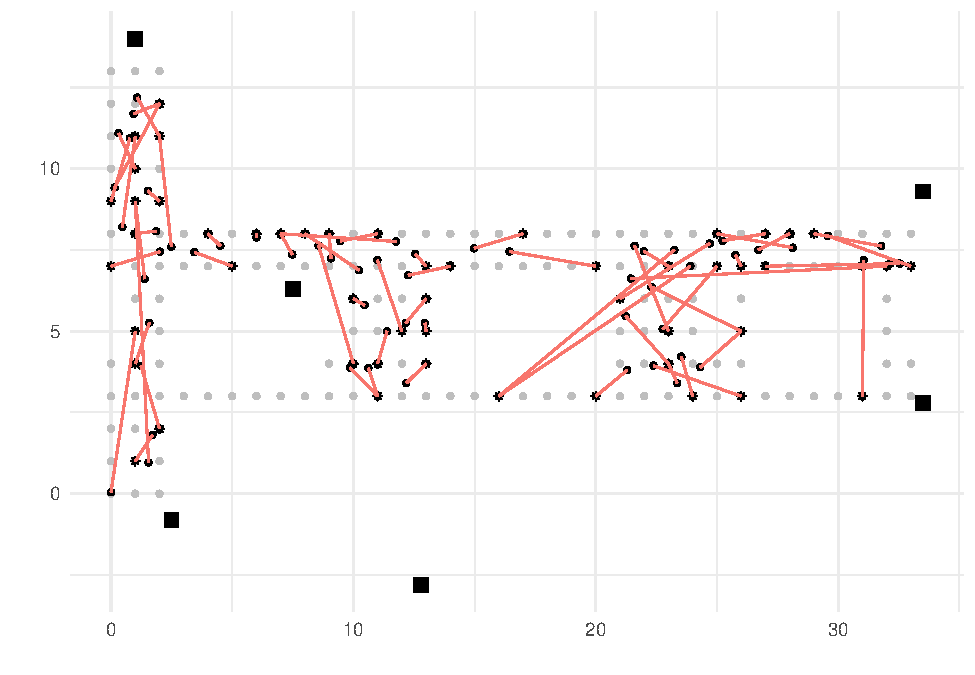
\includegraphics[width=0.8\linewidth]{Lab_Suplimentar_IPS_files/figure-latex/unnamed-chunk-52-1} \end{center}

\begin{center}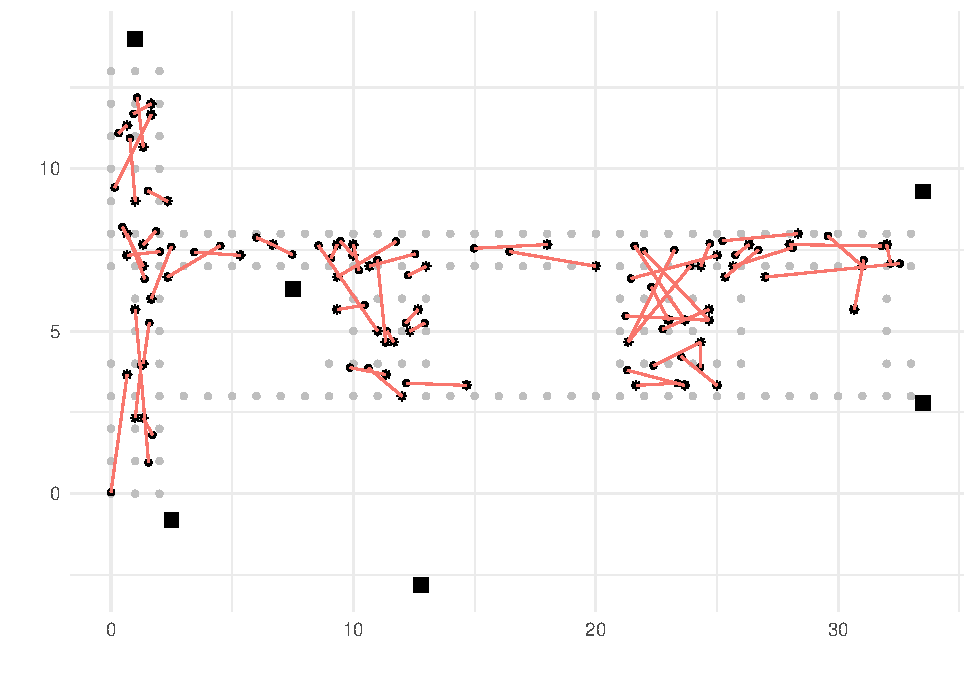
\includegraphics[width=0.8\linewidth]{Lab_Suplimentar_IPS_files/figure-latex/unnamed-chunk-52-2} \end{center}


\end{document}
